\chapter{Traffic Light Data for Prediction}\label{ch:prediction}

% TODO: Paper IV

\section{Introduction}

The fact that road users do not know when the traffic lights will change leads to several well-known problems. First, the issue of unneeded stopping and idling at red lights unnecessarily increases energy expenditure and emissions. In addition, not knowing about the upcoming traffic light's switching behavior also has negative impacts on road safety. There is a so-called dilemma zone when approaching a traffic light, where it unexpectedly turns yellow, and one must decide whether to stop before the light \cite{zhang_yellow_2014, suzuki_new_2018}. Often, this can lead to running a red light, speeding, or misunderstandings between drivers, increasing the overall risk of accidents.

Here, improved communication between vehicles and infrastructure elements could reduce the risk of accidents and traffic inefficiency \cite{sun_optimal_2020}. Such collaborative awareness is critical in current Cooperative Intelligent Transport Systems (C-ITS) research. Predicting traffic lights and communicating this prediction to vehicles, establishing the C-ITS day-1 service GLOSA, is one integral part of a more extensive portfolio of potential measures \cite{mellegard_day_2020}. Nonetheless, it is essential to consider that traffic light prediction is not strictly limited to GLOSA-like systems and may also lay the foundation for other application scenarios. For example, with the emergence of Augmented Reality, also in bike contexts \cite{matviienko_bikear_2022, kosch_notibike_2022}, there may be many more application scenarios than we currently envision.

Despite these encouraging prospects, traffic light prediction is currently associated with multiple challenges. Although countdown displays at traffic lights are widespread in various countries \cite{nygardhs_cyclists_2021}, integrating a mobile system to access and utilize the residual phase time directly from the traffic light's control unit presents a significant challenge. This process contrasts with the operation of countdown displays, which transfer the phase time internally to a countdown controller \cite{islam_improved_2016}.

A mobile system working across multiple intersections requires an interoperable data source. Here, the option exists to obtain the control programs directly, but without the current internal program state \cite{zweck_traffic_2013}. Since traffic-adaptive signals may only decide within a few seconds how long the next green phase will be switched \cite{islam_improved_2016}, this method is considered to be mainly restricted to fixed-time traffic light control programs that always switch in the same manner \cite{zweck_traffic_2013}. This is a strong limitation, as only 161 out of 1731 intersection controllers in Hamburg run a fixed-time program as of 2023\footnote{This information could be extracted from a traffic control inventory of the LSBG / IVS1 (as of June 22, 2023) provided on request, in addition to an inquiry to the Hamburg Senate: \url{https://www.buergerschaft-hh.de/parldok/dokument/72143/ampelschaltsysteme_gruene_welle.pdf}}. For the remaining 1570 traffic lights, we may expect interchanging or dynamic parts of the switching program.

Due to these issues, another method to access traffic light data has been established to deploy traffic light assistance services in the field. Most GLOSA applications use the residual time provided by Signal Phase and Timing (SPaT) messages generated on the intersection controller level and transmitted to the vehicle \cite{wagner_spatmap_2023}. However, such messages may only be available in some cases at the given location -- sometimes, as in this work, the prediction of traffic lights has to be performed purely by observing the outside state \cite{protschky_extensive_2014, protschky_adaptive_2014}. Furthermore, not all methods of traffic light data acquisition may be practical for smartphones.

In this work, we will utilize a centralized data broker, the Traffic Lights Data platform, that is provided by Hamburg authorities. However, a key challenge with these kinds of data platforms is the reliability of the traffic light data \cite{protschky_extensive_2014, protschky_adaptive_2014}. The state information may arrive incomplete, drop out completely for longer periods, or be highly delayed. These data issues impede the ability of the traffic light prediction to react to short-term changes in the program or may lead entirely to false and unavailable predictions. Quality assurance methods are required to identify these problems if they are present, and plan according solutions. This will be the first key challenge we will address in this chapter.

The second key challenge is the traffic-adaptiveness of traffic lights. Traffic-adaptive adjustments of switching programs are intended to improve the traffic flow at an intersection but have adverse effects on predictability due to short-term green time adjustments \cite{schweiger_elisatm_2011, bodenheimer_enabling_2014}. Recently, methods have been developed that focus on a more accurate prediction of traffic lights, but not all prediction methods may be equally suited for all kinds of traffic light patterns. Furthermore, some prediction methods may be more sensitive to data errors and outages than others. Thus, to understand precisely at which spot which prediction method is suited, the second main challenge of this chapter is developing a framework that helps in the decision process.

The goals of this chapter are to address these two challenges as follows. First, we will discuss the current methods to obtain traffic light data and which data issues may arise from centralized data infrastructures, as used in this work. Afterward, we will review state-of-the-art prediction methods and discuss their suitability for highly adaptive switching and highly erroneous data transmission. Based on this understanding, we will develop a twofold framework for traffic light data monitoring and data quality assurance. The first main component is monitoring methods that allow us to identify data issues and outages. Second, we develop metrics that can be used to measure the adaptivity patterns in traffic light switching and decide which kind of traffic light prediction may be suitable. Finally, we will evaluate the results of this framework and draw conclusions about how well traffic lights can be predicted in Hamburg with existing methods.

\section{Related Work}

To obtain a full picture of traffic light data and prediction, we will first look at studies designed to transmit traffic light data to traffic participants. These studies will provide a thorough understanding of the current data challenges behind GLOSA systems. Largely independent of these studies, multiple prediction methods that aim to improve prediction accuracy have been proposed. A discussion of these studies will help us learn the methods behind traffic light prediction and which issues may arise from a city-scale real-world deployment. Afterward, with the learnings from both domains, we will design a quality assurance framework for an existing data pipeline and prediction system in Hamburg.

\subsection{Data Challenges of Decentralized Systems}

In Europe, a large body of research and investments is currently flowing toward decentralized traffic light data systems, especially those based on Dedicated Short-Range Communication (DSRC). Road Side Units (RSUs) are deployed at intersections to operate these systems, sending standardized radio messages on the 5.9 GHz frequency band. These standardized C-ITS messages include SPaT messages, which vehicles can directly collect with a corresponding antenna (On Board Unit, OBU). A SPaT message contains the current switching state of a traffic light and a residual time until the next switch, making it an ideal data foundation for GLOSA applications \cite{ibrahim_estimating_2019, wagner_spatmap_2023}. Thus, many studies related to GLOSA utilize this data foundation \cite{schweiger_elisatm_2011, rakha_eco-driving_2011, rakha_aeris_2012, li_open_2012, suramardhana_driver-centric_2014, xu_bb_2015, bernais_design_2016, nguyen_efficient_2016, choudhury_integrated_2016, stahlmann_multi-hop_2017, stahlmann_exploring_2018, plianos_predictive_2018, zhang_green_2020, chen_developing_2022}.

SPaT messages are typically generated within the intersection controller level \cite{zweck_traffic_2013} and transmitted directly to an RSU without a centralized server system. However, such a system is typically not entirely decentralized. To calculate the residual time, there is the need for an additional prediction module, which may communicate with a cloud system in which a prediction algorithm is running \cite{strobl_c-its_2019, neuner_leitfaden_2020}. Due to the decentralized message transmission, however, a key advantage of this approach is that every vehicle equipped with a capable radio antenna has access to this data foundation. Thus, this approach is highly interoperable and attractive for manufacturers. The main per-unit cost factor is equipping intersections with the necessary RSUs \cite{niebel_cost-benefit-based_2013}.

A current research problem with decentralized approaches is the limited over-the-air radio transmission distance, especially when foliage blocks the line of sight. Since the 5.9 GHz frequency band resides closer to visible light's wavelength than other network carriers, such as 3G and 4G, it does not penetrate well through obstacles. In response to this issue, the C-Roads project, a prominent initiative in Europe's C-ITS landscape, submitted a statement advocating for the supplementation of the 5.9 GHz band with lower-frequency bands \cite{bohm_radio_2017}.

With DSRC only, Stahlmann et al. (2017) \cite{stahlmann_multi-hop_2017} show that obstacles may reduce the transmission range to less than 150 meters. The drop in the transmission rate is not immediate but gradual, which is why a partial message loss must always be assumed with this method. Sharara et al. (2019) \cite{sharara_impact_2019} provide more insights into the relation between packet loss, a GLOSA system's activation distance, and the speed advisory's effectiveness. The authors show that partial message loss of up to 90\% is not a significant problem unless the transmission distance is cut down too much, impacting the speed advisory system's activation distance and effectiveness. In a simulation with a minimum speed of 35 km/h, maximum speed of 75 km/h, specific green time of 25 seconds, red time of 40 seconds, and amber time of 5 seconds, Sharara et al. (2019) \cite{sharara_impact_2019} find that the transmission distance should be at least 850 meters for a 100\% success rate of traversing the green light, while 300 meters only resulted in 50\% -- 60\% of green passes depending on the message loss rate (90\% -- 10\%). Thus, with the transmission distance reported by Stahlmann et al. (2017) \cite{stahlmann_multi-hop_2017}, GLOSA services may occasionally fall short of their potential benefit simply because they are activated too late.

One explored solution to improve transmission range is an optimized RSU placement \cite{mehar_optimized_2015, massobrio_smart_2015, al-ezaly_optimal_2020}. Another option may be to adjust the transmission rate, which is reported in different ranges of 4 Hz \cite{stahlmann_multi-hop_2017} to 10 Hz in Hamburg \cite{stegen_ideas_2021}. The third option is inter-vehicle relaying of the messages to artificially expand the transmission range, as proposed by Stahlmann et al. (2017) \cite{stahlmann_multi-hop_2017}. Thus, a few practical solutions have already been presented to mitigate the limited transmission distance problem. For smartphone applications without direct access to an OBU, external antennas have been developed that can be connected via a USB cable \cite{kim_vulnerable_2017}. Additionally, manufacturers Bosch\footnote{\url{https://www.bosch-presse.de/pressportal/de/en/auto-cycling-and-tech-innovators-launch-coalition-for-cyclist-safety-based-on-v2x-deployments-259136.html}} and Canyon\footnote{\url{https://media-centre.canyon.com/en-INT/226588-canyon-plan-to-integrate-autotalks-v2x-technology-into-bicycles-to-help-reduce-accidents}} may introduce OBUs into their bike components soon, making this technology more accessible to cyclists.

One emerging alternative to 5.9 GHz radio is cellular vehicle-to-everything (V2X). This transmission technology utilizes an existing carrier medium such as 4G or 5G for the message transfer \cite{xia_field_2012, zweck_traffic_2013, bhattacharyya_assessing_2022}, distributing messages directly from an RSU (decentralized) \cite{bohm_radio_2017} or via cell towers (semi-decentralized) \cite{strobl_c-its_2019, jacob_ivs-kom_2020}. Although this carrier medium is interoperable on the application level (transmitting SPaT messages), there seem to be incompatibility issues on the network level \cite{bohm_radio_2017}. Thus, while DSRC is widely deployed on roads in Austria and Germany\footnote{\url{https://auto-talks.com/technology/dsrc-vs-c-v2x/}}, cellular V2X is seen by some experts to replace DSRC in the future\footnote{\url{https://www.cloudflight.io/en/blog/5g-killer-app-v2x-requires-the-transformation-the-automotive-industry/}}. Amid this uncertain state, C-ITS pilots \cite{strobl_c-its_2019} and OBU manufacturers \cite{jacob_ivs-kom_2020} develop multi-band solutions working with cellular V2X and DSRC in parallel.

Another issue is the unclear long-term compatibility of cellular V2X with smartphones. Not much research could be found in this direction, so we have to base our observation on technical documents. Although chipsets exist that enable LTE-V2X through the PC5 mode (direct device-to-device communication) and LTE-V2X/5G-V2X via cell towers\footnote{\url{https://5gaa.org/content/uploads/2021/11/5GAA_List_of_C_V2X_devices.pdf}}, these chipsets seem to be manufactured mainly for automotive applications. The 5G Automotive Association, a proponent of cellular V2X encompassing automotive and chipset manufacturers, predicted LTE-V2X in 2017 to penetrate 80\% of new smartphones by 2027\footnote{\url{https://5gaa.org/content/uploads/2017/12/5GAA-Road-safety-FINAL2017-12-05.pdf}}. However, this prediction is based on an optimistic scenario in which smartphone manufacturers react to increasing demand for C-ITS applications induced by LTE-V2X deployments in cars. There is also the pessimistic scenario in which 0\% of smartphones will support this technology in the future. Currently, it is up for speculation which scenario is more likely, meaning that cellular V2X is not yet an established data source for smartphone-based GLOSA applications.

\subsection{Data Challenges of Centralized Systems}

While DSRC and cellular V2X aim to provide a near-range network for C-ITS message communication, there is also the option for a traditional approach over the Internet. With this approach, the traffic light data is collected at a centralized server infrastructure located near the traffic management center and redistributed over an internet endpoint \cite{zweck_traffic_2013, protschky_extensive_2014, protschky_adaptive_2014}. In this way, a centralized traffic light data infrastructure circumvents two challenges of decentralized approaches: limited transmission range and long-term compatibility with smartphones. However, as we will see, it also shifts the responsibility of interoperability, data processing, and quality assurance toward the service consumer.

At Audi, Zweck et al. (2013) \cite{zweck_traffic_2013} established a data foundation for a GLOSA system that ingests traffic light data from three major cities. Correspondingly, three data adapters needed to be implemented: In Verona, the car manufacturer had access to SPaT messages generated on the intersection controller level. In Garmisch, intersection controllers were retrofitted with an additional SWARCO forecast module to obtain the necessary data, presumably SPaT messages. In Berlin, multiple traffic control centers were connected with various protocols, for which the specific transmission format is not further disclosed. The implemented data adapters were integrated into a centralized proprietary backend of Audi, making the corresponding traffic light information available to the company's vehicles via a mobile network connection to the internet. Unfortunately, the specific prediction methods and challenges related to traffic light prediction are not provided in detail. While it is generally unclear where this system is currently in operation, the available information indicates that the system was introduced in the United States in 2016 and was utilized at least until 2020 to facilitate Audi's GLOSA services in Düsseldorf \cite{neuner_leitfaden_2020}.

Many studies, whether decentralized or centralized, utilize the contained prediction in SPaT messages directly to generate the GLOSA service without needing an additional prediction system. In this way, these studies delegate the task of traffic light prediction to the infrastructure provider. However, some occasions may lead to the circumstance that the SPaT messages are not directly processable or available. The stability of the messages may also not be guaranteed at all times. Thus, it may be necessary to develop a custom prediction service that handles the available data formats and is robust to data outages, as shown by Protschky et al. (2014) \cite{protschky_extensive_2014, protschky_adaptive_2014}. In their studies conducted for BMW, the authors were confronted with multiple traffic light data issues in Munich. Usually, the delays in traffic light messages are within a few seconds \cite{neuner_leitfaden_2020}. However, in Munich, the authors had to work with SPaT messages arriving 10 to 60 minutes late from the city's data system. This significant delay meant that the residual prediction contained in the SPaT messages would be far outdated once the backend obtained this information. Furthermore, the traffic light messages were also partially incomplete.

Protschky et al. (2014) \cite{protschky_extensive_2014, protschky_adaptive_2014} approached the challenges as follows. First, they recorded the traffic light states contained in the SPaT messages, storing the data in histories for each traffic light. Afterward, they extrapolated the seen patterns in the historical data until the current time and slightly beyond to derive a prediction. In this way, the prediction was decoupled from the significant delays. When detecting that the prediction would no longer correlate with the actual observed data to over 95\% accuracy, as required by BMW, the prediction was turned off for the affected traffic lights. While the authors had to cope with significant data issues, their approach achieved a reported prediction availability of at least 69\%. Thus, while not all traffic lights could be predicted at all times, and the message delays likely imputed adaption to short-term changes in the traffic light behavior, the authors could still achieve a functional large-scale prediction system.

Compared to decentralized systems, centralized approaches to obtaining traffic light data are more compatible with smartphone applications and are still utilized today by at least one large car manufacturer. However, an ongoing challenge is to overcome the data issues of these systems. Protschky et al. (2014) \cite{protschky_extensive_2014, protschky_adaptive_2014} present a prediction method that even works when the data is highly delayed or incomplete. However, it must be expected that not all traffic lights will provide a prediction, as data errors may decrease the prediction availability.

\subsection{Traffic-Adaptive Signal Timing}

Due to the increased availability of traffic light data, it also becomes more viable to develop more intelligent coordination of the switching behavior at intersections. As shown by Wang et al. (2018) \cite{wang_review_2018}, a key research goal in traffic control is to develop more advanced coordination strategies for traffic lights, reducing unnecessary congestion. However, a more active traffic light control also means that passive assistance systems like GLOSA become more challenging. Thus, as discussed by Otto et al. (2023) \cite{otto_framework_2023}, both kinds of research actively work against each other. Different prediction approaches have been presented to counteract the issue of traffic adaptive signal timing for GLOSA systems. 

\begin{figure}[t]
\centering 
\begin{tabular}{ccc}
\footnotesize{(a) Fixed-time} & \footnotesize{(b) Partially adaptive} & \footnotesize{(c) Fully adaptive} \\
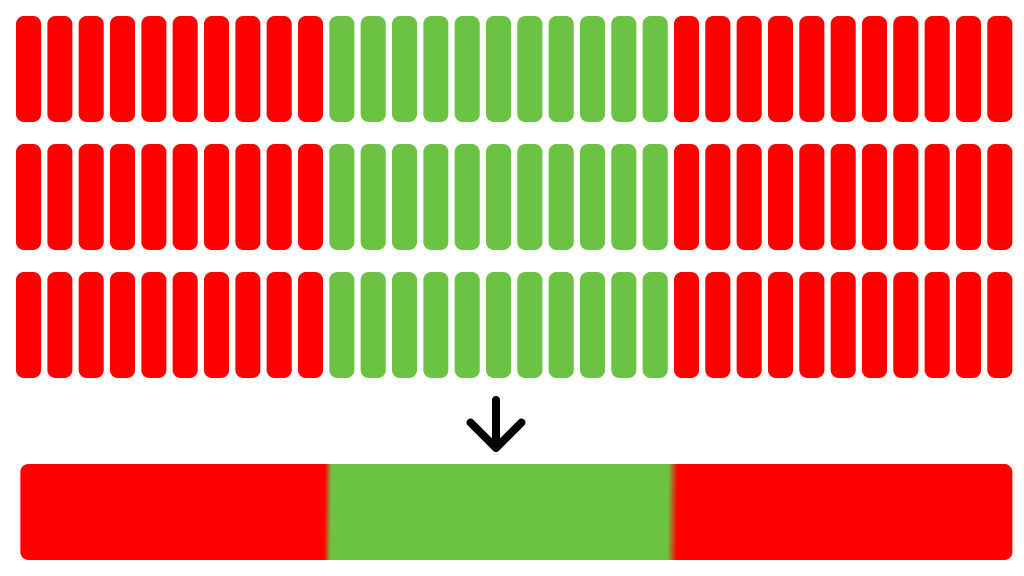
\includegraphics[width=0.3\linewidth]{images/explanation-fixed-time.png} & 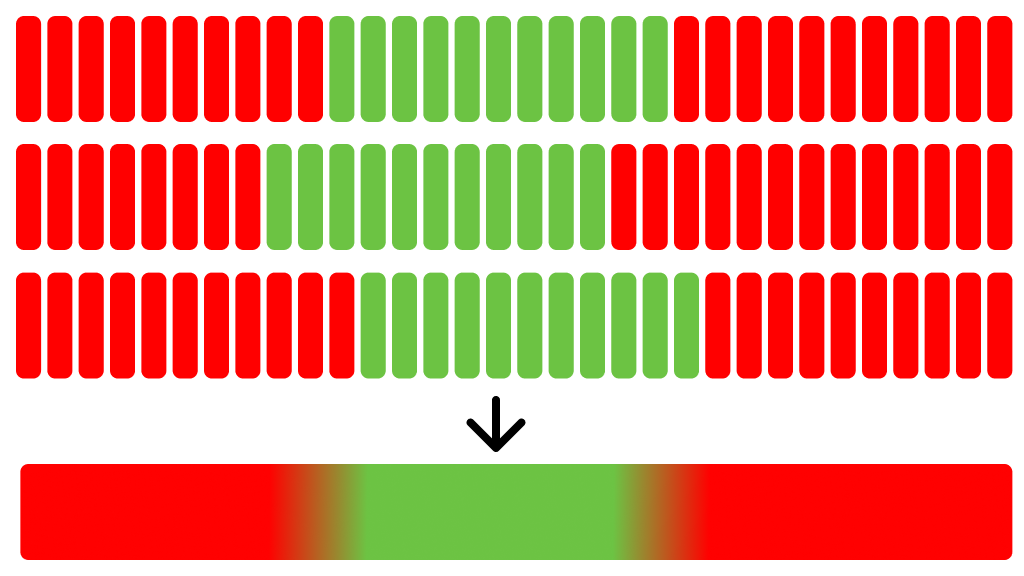
\includegraphics[width=0.3\linewidth]{images/explanation-partially-adaptive.png} & 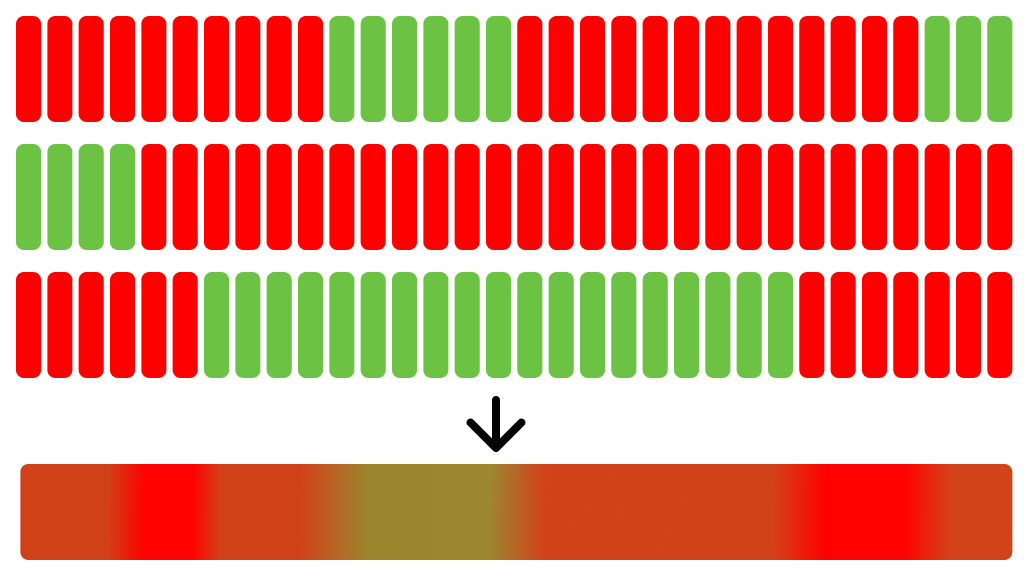
\includegraphics[width=0.3\linewidth]{images/explanation-fully-adaptive.png}
\end{tabular}
\caption{Taxonomy of the three types of traffic light adaptivity. Seen are the traffic light program cycles that contain the switched colors. On the bottom, we see a probabilistic prediction generated from the cycles and how the different types of adaptive switching behavior influence it.}
\label{fig:prediction}
\end{figure}

The first idea to address adaptive timing is to add probabilities to a traffic light prediction. With this approach, each second in the prediction is associated with a probability that the color will be seen at this moment, depending on previous switching behavior. This approach is illustrated in \Cref{fig:prediction}, and was initially proposed by Protschky et al. (2014) \cite{protschky_extensive_2014, protschky_adaptive_2014}. First, full circulations of the traffic light's program (cycles) are recorded and aligned in history. Alignment is performed with information on when a new cycle was started. Afterward, the probability of "green" and "red" is determined for each second through the prevalence of the predicted color at this specific second in previous cycles. Since the adaptive component is represented as a probability, the speed advisory can focus on certain parts of the prediction, counteracting the adaptive behavior. As a result, this kind of prediction algorithm reacts to traffic adaptive signal timing by blurring out uncertain parts of the prediction. 

With this approach, the speed advisory algorithm must decide which prediction parts are considered safe enough. One potential solution was introduced by Mahler et al. (2012) \cite{mahler_reducing_2012}, who showed possible optimization methods for calculating the optimal speed with an uncertain prediction. A recent work by Typaldos et al. (2023) \cite{typaldos_modified_2023} has further developed the idea of calculating a probabilistic/stochastic speed advisory. However, one intrinsic challenge of this approach is that, as adaptability increases, it tends to converge more towards the midpoint of the green phase. Following the speed recommendation may result in the vehicle not reaching the traffic light precisely on time but instead with some delay. Thus, from the standpoint of minimizing unnecessary braking as much as possible, the speed advisory is not necessarily "optimal."

Another idea explored in related works is to adjust the prediction in real-time to the observed traffic light states, stretching or shortening the predicted residual time when unpredicted changes happen. Such self-adaptive prediction methods have been initially proposed by Bodenheimer et al. (2014 -- 2015) \cite{bodenheimer_enabling_2014, bodenheimer_glosa_2015} through a graph-based method. Their method observes the ingress directions at an intersection node and reconstructs the relation between the clearance timing of each direction. Schneegans et al. (2023) \cite{schneegans_prediction_2023} also demonstrate the possibility of utilizing Machine Learning models for this process. Here, the idea is to utilize a sequence prediction model trained on prerecorded timing data from a specific traffic light. In general, self-adaptive methods, and especially methods based on sequence prediction, seem to be a recent trend in achieving higher accuracy, following the success of Machine Learning in other domains.

However, self-adaptive methods are not without criticism. As pointed out by Stahlmann et al. (2018) \cite{stahlmann_exploring_2018}, the stretching and shortening of the prediction can also be seen as a significant disadvantage of this approach. Since repeated adjustments to the prediction during the intersection approach may negatively impact usability, there is a clear tradeoff between the prediction's accuracy and temporal stability. The increased computational complexity of the presented Machine Learning models is also a factor that may negatively impact the prediction algorithm's scalability toward multiple thousand traffic lights. There is currently no evidence supporting the scalability on a large scale as opposed to probabilistic approaches \cite{protschky_extensive_2014, protschky_adaptive_2014}. 

Furthermore, while the probabilistic approach is intrinsically robust to incomplete data and can drop individual cycles, error robustness is another factor to consider in evaluating self-adaptive models. These challenges must be addressed to employ such a model in practice. Most importantly, however, the traffic light data must arrive in time for the self-adaption to happen. Thus, self-adaptive prediction methods can only be employed when the traffic light data arrives with low latency, posing a significant limitation for real-world deployments. In a situation such as reported by Protschky et al. (2014) \cite{protschky_extensive_2014, protschky_adaptive_2014} where traffic light messages may arrive with a delay of over 10 minutes, a self-adaption would be basically useless.

In general, the issue of traffic adaptivity is not fully solved yet, with limitations in both probabilistic and self-adaptive prediction methods. However, the necessity to address this issue also depends on the extent to which traffic adaptivity is actually present in the real world. Here, various reports can be found.

Cai et al. (2009) \cite{cai_adaptive_2009} were the first to report that "most" traffic lights in their context are traffic-adaptive. Concrete numbers were presented by Bodenheimer et al. (2014) \cite{bodenheimer_enabling_2014}, who reported that 95\% of traffic lights in Hamburg were adaptive and 73\% in the ten largest German cities. Fakler et al. (2014) \cite{fakler_structures_2014} also found a high proportion of traffic-actuated control systems in German cities with over 50000 inhabitants. Schneegans et al. (2022) \cite{scheegans_exploiting_2022} and Heckmann et al. (2023) \cite{heckmann_stage_2023} further support the conclusion that most traffic lights are operated by traffic-adaptive controls. Hao et al. (2019) \cite{hao_eco-approach_2019} noted the widespread deployment of actuated traffic light controllers in the US, while Avatefipour and Sadry (2019) \cite{avatefipour_traffic_2018} found that fixed timing is more prevalent in Malaysia. Grumert and Pereira (2022) \cite{grumert_heads-up_2022} found that 70\% of traffic lights in Sweden are adaptive. Thus, there seem to be regional differences in the implementation.

Unfortunately, we found no global studies based on reliable sources that investigate the employment of traffic light adaptivity by country. Only one study by Olaverri-Monreal et al. (2018) \cite{olaverri-monreal_implementation_2018} could be found that did not clearly refer to a specific region. The authors report that adaptive timing is only implemented in a small number of road networks, and the majority of urban areas still use pre-timed control systems. However, how reliable this information can be considered is not fully clear, as a source for this finding was not provided. A similar issue also applies to other studies. For example, in the work by Bodenheimer et al. (2014) \cite{bodenheimer_enabling_2014}, which mentions 95\% adaptive traffic lights in Hamburg, it was only clarified upon inquiry that these results were based on a survey conducted by a service provider on behalf of Audi. The study by Grumert and Pereira (2022) \cite{grumert_heads-up_2022} provides a Swedish source for their findings, but we were unable to find it. Hence, we have to be intrinsically skeptical about these reports.

Based on the information we have, Germany seems to utilize traffic-adaptive signals predominantly. Findings for Hamburg roughly align with our analysis that counted 90.7\% (1570 out of 1731) adaptivity-capable traffic light controllers. However, aside from the general lack of verifiable results, the implications for predictability remain largely unexplored. While the capacity to adapt to traffic may exist, it might be underutilized or manifested only in minor adjustments, potentially resulting in a less significant impact on prediction accuracy, as indicated by the reported percentages. Presently, no study examines the real-world effects of adaptiveness on predictability, leaving a significant research gap.

\begin{Summary}[Summary of Research Gap]
While many works focus on decentralized data transmission, a centralized approach is currently the best option for cyclist applications. Most centralized platforms provide an endpoint for SPaT messages generated at the intersection controller level. Based on this endpoint, the residual time prediction in SPaT messages can be directly used for a speed advisory application.

In cases where no SPaT messages are available or arrive too late, the best approach involves recording switching histories, running a suitable prediction algorithm on these histories, and sending the generated predictions to service users. Data latencies can be circumvented through an appropriate prediction approach, such as a probabilistic method. Nonetheless, there are only few works on the data challenges on a larger scale, thus requiring more research. Existing works indicate significant issues with data reliability that must be accounted for.

Furthermore, it is unclear at which intersections novel prediction methods such as machine learning models may provide a better prediction than the existing probabilistic method. Although machine learning methods may have advantages and provide a more self-adaptive prediction, issues like unproven robustness against data errors, scalability, and the temporal instability of the predicted residual time mean that we have to carefully consider at which crossings these methods should be applied. 

While some studies pose traffic-adaptive switching behavior as their central motivation to develop more advanced prediction methods, it is unclear how justified these motivations are. Reported numbers of adaptive traffic lights provide a rough estimate but no definite conclusion about the actual predictability of traffic lights. If adaptiveness is seen but is limited to a few seconds, it may necessitate reevaluation of developed prediction algorithms. Here, a direct analysis of traffic light data is needed to determine how many traffic lights exhibit adaptive behavior and how much this behavior impacts predictability.
\end{Summary}

\section{Concept}

We will conduct two steps to address the described research gaps. First, we will design a quality assurance framework that monitors data availability and potential errors, at the example of our traffic light data infrastructure in Hamburg. The goal is to provide quality assurance solutions to improve the prediction that GLOSA app users can expect as much as possible. Using a monitoring infrastructure, we will conduct a large-scale, long-term study on the prediction availability and quality. As a prediction method, we reuse the existing probabilistic prediction method, with the goal of identifying potential weaknesses and advantages of that method in our field deployment and how reliable traffic light data is.

Second, we address the need for more research on traffic light adaptiveness and predictability. In contrast to previous studies, we attempt to measure the predictability directly, and identify which kinds of prediction algorithm may be applicable at each intersection. To conduct such a study, we first collect large amounts of traffic light data. Afterward, we design and evaluate two novel metrics that help us measure which kinds of prediction methods may be applicable. The goal is to provide the first large-scale insights into the kinds of traffic light patterns that are seen in a large city such as Hamburg and thus clarify how much traffic adaptivity is a concern for traffic light prediction.

\subsection{Prerequisites: Existing Data and Prediction Infrastructure}

Before we focus on our data quality assurance methods, we briefly look at the existing data and prediction infrastructure, on which we will apply our monitoring and analysis.

To bring forward intelligent transport solutions such as GLOSA applications, Hamburg employs an open data policy through its self-imposed transparency law (HmbTG\footnote{\url{https://transparenz.hamburg.de/gesetzestext-des-hmbtg-636070}}), providing several kinds of urban data free of charge to the public. Hamburg provides static, continuously updated, real-time datasets and geo APIs as part of this urban data platform. One of these APIs is the Traffic Lights Data\footnote{\url{https://metaver.de/trefferanzeige?docuuid=AB32CF78-389A-4579-9C5E-867EF31CA225}} system, which provides real-time information about the switching of traffic lights in Hamburg and georeferences their location in the city. Published by the Free and Hanseatic City of Hamburg, Landesbetrieb Straßen, Brücken und Gewässer (LSBG), the data is made available under the DL-DE BY-2.0\footnote{\url{https://www.govdata.de/dl-de/by-2-0}} license and will be considered the foundation of this work.

One challenge of using the Traffic Lights Data platform for prediction and speed advisory in a GLOSA application is that the state messages are not provided in the SPaT format. Thus, no residual time prediction, as contained in SPaT messages, is available, meaning that we have to implement an external prediction service to establish our GLOSA service. Changes in each traffic light's state are provided as real-time observations through the SensorThings\footnote{\url{https://www.ogc.org/standard/sensorthings/}} "Observation" format. Besides vehicle detector or bus request messages, three particular types of messages represent the foundation for our prediction:

\begin{itemize}
    \item \textbf{(Primary) signal color}: the current traffic light color and the time when this color was switched. Among green, red, amber, and amber-red, there are also other specific states such as amber-flashing, green-flashing, or dark (light turned off). The color is given for the primary signal head and supplementary signals, such as green arrows.
    \item \textbf{Signal program}: the current program ID running on the traffic light, with a time when this program was switched.
    \item \textbf{Cycle second}: a timestamp indicating that program recirculation has happened. With this timing information, the continuous stream of colors can be split into cycles, usually 90, 75, or 60 seconds long. This information is also given for traffic lights that do not strictly use a circulating program routine.
\end{itemize}

The Traffic Lights Data platform was designed based on an existing traffic controller infrastructure and implemented by various stakeholders. The system design of the platform follows these technical and organizational constraints, resulting in a rather complex chain of information. As we will later see, precisely understanding this chain of information is crucial to tracing data issues that may arise. Thus, through dialogues with various authorities in Hamburg, we reconstructed a precise picture of the infrastructure and potential points of failure.

\begin{figure}[t]
\centering
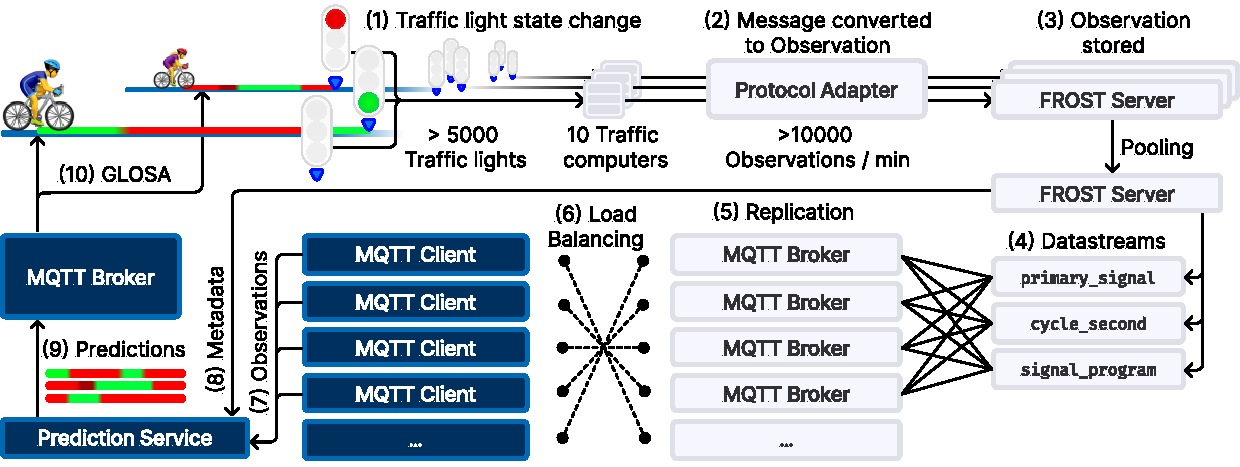
\includegraphics[width=\linewidth]{images/traffic-light-data-infrastructure.pdf}
\caption{Data flow diagram of the existing traffic light data infrastructure. Highlighted in grey are the components of the Traffic Lights Data infrastructure. Blue components highlight our implemented data adapter and prediction services.}
\label{fig:traffic-light-data-infrastructure}
\end{figure}

To provide state messages in the Traffic Lights Data platform, they are translated and shifted multiple times between various data brokers. First, as seen in \Cref{fig:traffic-light-data-infrastructure}, the state messages are sent in a controller-specific format to one of ten traffic controllers (1). Then, the messages are converted to Observations (2) and sent to a corresponding SensorThings server. From there, a centralized SensorThings server collects all Observations (3), which are associated with a specific type of "Datastream" encapsulating the type of Observation: \texttt{primary\_signal} (color), \texttt{cycle\_second}, and \texttt{signal\_program} (4). Finally, the messages are published across an autoscaled Kubernetes cluster of MQTT brokers (5). 

Afterward, our prediction service connects to the broker endpoint to ingest all Observation messages. Our prediction service utilizes multiple MQTT clients with individual TCP connections to balance the load on each MQTT broker in the Traffic Lights Data platform (6). The collected Observations (7) are combined, knowing which Observation is associated with which traffic light through metadata in the Traffic Lights Data platform (8). This metadata allows the prediction service to record a history of program cycles and associate it with the corresponding traffic light ID. Based on these histories that are continuously updated, the prediction algorithm runs periodically to keep predictions up to date (9). 

The prediction algorithm itself was implemented by Sebastian Pape based on the method developed in his Diploma thesis \cite{pape_untersuchung_2012} and integrated into the data pipeline with corresponding programming interfaces. The programming interface converts the Observations into an internal format for the prediction algorithm, meaning that the programming interface is interoperable with other message formats as long as the three described types of traffic light state messages are given. Based on this foundation, the existing implementation could be seamlessly ported to other cities that provide the desired messages.

At its foundation, the integrated prediction method is equivalent to the probabilistic method by Protschky et al. (2014) \cite{protschky_extensive_2014, protschky_adaptive_2014}. It reconstructs cycles based on the cycle timing information and calculates which color will most likely appear for each second. To allow the prediction algorithm to adapt to changing programs, only the last ten cycles are kept for prediction. Then, every 60 seconds, the current history of each traffic light is fetched, and a new prediction is calculated based on the current time. The prediction is extrapolated to be 180 seconds long. This extrapolation will allow our app to display an appropriate speed advisory even when users are far from the traffic light. 

Each prediction also contains a prediction quality. This value will become crucial for our monitoring and quality assurance, as it determines how accurately the prediction fits the real observed states. After creating a new prediction vector $P$ that consists of predicted second-wise colors, it is held for 120 seconds. Then, each second in the collected data vector $D$ containing the actual second-wise colors is compared to the prediction $P$, calculating an accuracy score:


\begin{equation} 
\text{Prediction Quality}(D, P) = 
\frac{
\sum_{i=0}^{119} 
\left\{
\begin{array}{ll}
1 & \text{if } D[i] = P[i] \\
0 & \text{otherwise}
\end{array} 
\right.
}{
120
}
\end{equation}\label{eq:predictionquality}

This equation is based on work of Sebastian Pape \cite{pape_untersuchung_2012}. Note that the traffic light states in $D$ were not yet used to generate the evaluated prediction $P$, meaning the prediction is validated on unseen data. The calculated quality is then attached to the newly generated prediction, and the time when the quality was created is noted. If no full 120 seconds of real-time data are available for the validation, no quality is calculated. This means that, in the case of a data outage, the quality is not refreshed. After 10 minutes, when the quality cannot be refreshed, it is set to -1 to indicate that validation is no longer possible. 

After the prediction is generated and annotated with the current quality, it is published on an MQTT broker under the traffic light's ID, where the app is subscribed and automatically obtains new information. The prediction MQTT broker is configured to retain all messages, meaning that a new app subscription directly sends the last prediction for the subscribed traffic light. Finally, the app utilizes the obtained prediction to display a speed advisory.

\subsection{Data Quality Assurance}

\begin{figure}[!b]
\centering
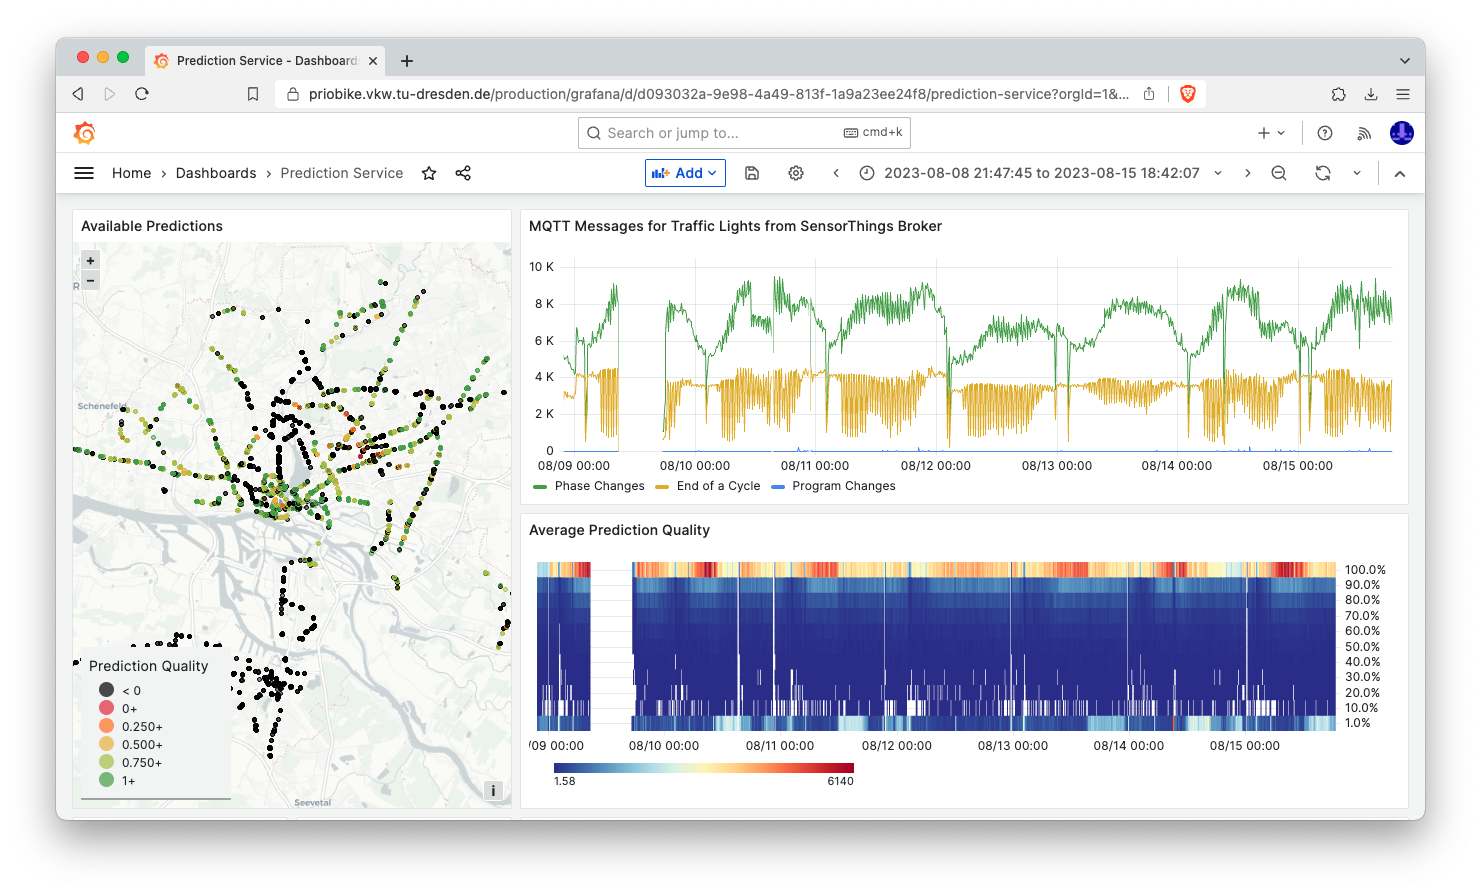
\includegraphics[width=\linewidth]{images/monitoring-screenshot.png}
\caption{Screenshot of the developed monitoring solution. Within the Grafana dashboard, three key aspects of data quality can be observed: the number of messages (top right), the distribution of prediction quality (bottom right), and the quality of predictions throughout the city (left).}
\label{fig:monitoring-screenshot}
\end{figure}

After having gained a thorough understanding of our existing data infrastructure, we can now focus on the key concepts for data quality assurance. First, we develop a web tool for prediction quality and data availability monitoring. This solution, shown in \Cref{fig:monitoring-screenshot}, is based on a web dashboard that highlights real-time metrics such as the number of Observations, generated predictions, and spatial distribution of the measured prediction qualities. At its foundation, this tool makes extensive use of the prediction quality metric that is associated with each generated prediction.

By viewing the prediction quality on a map, especially qualities mapped to -1 (highlighted in black), we can directly identify whether an outage is related to a specific traffic controller or associated with the complete city. If all city districts are affected, the problem is more likely to originate from the data pooling or load balancing components further along the information chain. 

Furthermore, we can study the time and duration of error patterns, giving us and the system's operators more clues about where to look for data issues. This aspect is depicted in the chart above which contains the number of traffic light messages, as well as a heatmap of the prediction quality that is measured for all traffic lights. The idea of the displayed heatmap is to detect unexpected drops in the prediction quality that happen over multiple traffic lights at the same time. Based on -1 states in the prediction quality, we can also see when a data outage occurs or when the traffic light turns itself off.

In addition to these simple metrics, we also measure the number of invalid cycles, referring to cycles that contain invalid transitions between traffic light phases. Specifically, we check if a recorded cycle deviates from the regular switching patterns red--red-amber--green--amber and red--green. We check the length of amber against its maximum duration of 6 seconds, together with the maximum red-amber duration of 2 seconds, as specified by German traffic light operation constraints \cite{TN_libero_mab2}. Detected erroneous cycles are then discarded before they are input into the prediction algorithm and logged by the monitoring system to identify outbreaks of erroneous data.

Although quite simple, the developed monitoring allows us to identify and report data failures to the platform operators based on discarded erroneous cycles, drops in the number of Observation messages, or a decreased prediction quality. Error patterns in the dropped messages allow us to provide more detailed information about the potential origins of data failures within the system's architecture. We deploy this system into our existing data and prediction infrastructure, adding one more monitoring instance at an external cloud provider to cross out issues from our TU Dresden deployment.

\subsection{Predictability Metrics}

Based on the same data pipeline, we conduct our predictability analysis. However, instead of collecting the data to generate predictions, we use it to measure the absence or presence of predictable patterns. To achieve this distinction, the idea is to measure how "noisy" the switching patterns are. The more random noise is seen in the switching behavior, the less predictable the traffic light.

Until we arrived at our final metrics, we investigated various methods from other disciplines to measure noisiness. For example, one idea was to measure the Shannon entropy of the traffic light's data stream, indicating how much information content and, thus, complexity of the switching behavior is present. Similarly, we attempted to use compression techniques to find how much information content is in the traffic light program. Another idea was to utilize a fast Fourier transform to find how many different frequencies in the switching patterns were present, mapping states between green (1) and red (0)\footnote{A future avenue of this approach could be to employ other methods for period detection in the switching patterns \cite{breitenbach_method_2023}. Such an approach was not tested as part of this work.}. However, in the end, none of the attempted methods yielded a satisfactory measurement of how many predictable patterns were present while comparing the calculated values against case studies. 

Based on the learnings from these methods, we approached the challenge with two more direct measurements that each indicate one simple kind of unpredictability. The first metric is based on the difference between recorded cycles. If there were traffic light colors that appeared at different times in the cycles, this would directly indicate a kind of traffic adaption. We gave this metric the name cycle discrepancy, calculated between two recorded cycles $C_1$ and $C_2$ being lists of second-wise traffic light states each, with the lengths $l_1 = |C_1|$ and $l_2 = |C_2|$:

\begin{equation} \text{Cycle Discrepancy}(C_1, C_2) =  \sum_{i=0}^{\max(l_1, l_2)-1} \left\{
\begin{array}{ll}
1 & \text{if } i \geq l_1 \text{ or } i \geq l_2 \\
1 & \text{if } C_1[i] \neq C_2[i] \\
0 & \text{otherwise}
\end{array} \right.\end{equation}

The cycle discrepancy is zero in cases when colors perfectly align between cycles and cycles have the same length. However, for example, if the green phase in one cycle appears and ends one second earlier than in the last cycle, the cycle discrepancy is calculated at two seconds. Thus, the more shift is seen between two cycles, the higher our cycle discrepancy. When a high discrepancy between two cycles is seen, this also indicates a high traffic adaptivity in the switching behavior. Note also the similarity to \Cref{eq:predictionquality}, which is intentional.

The cycle discrepancy assumes that green phases are aligned with the cycle length, meaning they appear at the same time every cycle. However, there may also be traffic lights where the waiting time between green phases is not aligned with the cycle timing. While the waiting time could be consistent and, thus, predictable, the cycle discrepancy would be high due to the misalignment. Hence, we designed a second metric that captures how many different wait times are seen. If all waiting times differ, this also indicates a high traffic adaptivity without being bound to the cycle length.

We name this metric the wait time diversity and calculate it as follows. First, the recorded cycles are concatenated into a continuous history $H_{C_1, \dots, C_n}$ of traffic light switching. Then, between every two green phases for which a continuous record is present, the wait time in between is measured and rounded in seconds. As a result, we obtain a list of wait times between green phases. Then, we measure how many \textit{different} waiting times are seen proportionally to the number of all wait times:

\begin{equation}
\text{Wait Time Diversity}(H_{C_1, \dots, C_n}) = \frac{\text{\# Different Wait Times}}{\text{\# Total Wait Times}}
\end{equation}

If there are reoccurring green patterns in the wait time, the wait time diversity is expected to be close to zero. If the variability of waiting times between green phases is high, and thus the number of different wait times, the wait time diversity is expected to be close to one. In the extreme case that only one green phase in the complete history is detected, the metric is set to one, meaning no reoccurring pattern was detected. If no green phase is detected, the metric is set to zero, assuming this represents an easily predictable pattern (always red).

Since the wait time diversity does not necessarily capture the amount of shift between green phases and only the uniqueness, both measures need to be employed in conjunction to determine whether predictable patterns are present.

\definecolor{good}{HTML}{00bb00}
\definecolor{bad}{HTML}{ff0000}
\begin{table}[!b]
\centering
\def\arraystretch{1.5}
\caption{Types of predictability mapped by our two metrics. This schema can be utilized to determine which kind of prediction algorithm may be suitable.}
\label{tab:cases}
\begin{tabular}{c|c|c|}
\multicolumn{1}{c}{} & \multicolumn{2}{c}{Cycle Discrepancy} \\
\cline{2-3}
Wait Time Diversity& Low& High\\
\hline
\multicolumn{1}{|c|}{High}& \textbf{\color{good} High predictability}$^1$& \textbf{\color{bad} Low predictability} \\
\hline
\multicolumn{1}{|c|}{Low}& \textbf{\color{good} High predictability}& \textbf{\color{good} High predictability}$^2$\\
\hline
\multicolumn{3}{l}{$^1$\footnotesize{Unpredictable wait time between green phases.}} \\
\multicolumn{3}{l}{$^2$\footnotesize{Unpredictable with our cycle-stacking (probabilistic) prediction method.}}
\end{tabular}
\end{table}

As a result, we obtain a measurement model that focuses on four cases, as visible in \Cref{tab:cases}. Whenever both measurements are low (bottom-left), the predictability is likely high with any of the currently available prediction methods, as each cycle tends to match with the next one, and the times between green phases also revolve. Similarly, when both measurements are high (top-right), the traffic light is likely poorly predictable, likely exhibiting highly spontaneous switching behavior. 

A more differentiated evaluation is necessary in cases where only one of both metrics is high. High cycle discrepancy in the presence of a low wait time diversity (bottom-right) indicates that our selected probabilistic prediction method should be avoided. It indicates that cycles are offset or non-matching, meaning that a cycle-stacking prediction algorithm will encounter intense blurring of the predicted colors. 

On the other hand, if the cycle discrepancy is low and the wait time diversity is high (top-left), the wait time between green phases is not well predictable, while cycles are similar. This may be the case when the traffic light only occasionally switches to green and shows red for the longest time. In this case, predicting red would be an accurate prediction in almost all cases, even though a green phase may occur at some point.

To apply this set of metrics to the traffic light data in Hamburg, we reuse the same data infrastructure as proposed earlier. However, we apply minor modifications to obtain more reliable measurements. As an additional error detection metric, we filter out all cycles that are 50\% longer or shorter than the previously recorded cycle length. This error metric aims to avoid too long or too short cycles skewing the final measurement, as they would boost the cycle discrepancy metric.

We also aim to minimize the noted problem of dropped Observation messages from the MQTT streams. Since the completeness of the messages is more critical for our predictability study than their timeliness, we can apply a workaround to get many more Observations than possible with MQTT only. We query all Datastreams in a round-robin fashion via the HTTP interface of the Traffic Lights Data API and fetch the latest Observations via this web interface. If we encounter any unseen Observations, we insert them into the database in which our MQTT Observations are located. 

Although theoretically applicable to the prediction service, this process is likely not an option for supplementing the real-time data during the traffic light prediction. Browsing through data streams via the HTTP interface takes a few minutes per roundtrip, meaning we would have to delay our MQTT Observations or adjust the reconstructed cycles artificially, which was not seen as sensible with the given algorithm implementation, although theoretically viable. Therefore, this approach was only applied in the data recording phase, which does not rely on sequential and minimally delayed Observations. Not integrating the complex HTTP queries into our prediction service also means the Traffic Lights Data platform does not have to deal with a continued disproportionate load after our experiment is finished.

During our experiment, the recorded data of all traffic lights is stored in a Postgres database. However, due to the large number of messages obtained, we also employ some optimizations to the data storing and database fetching process. During analysis, we group the received data into hourly buckets, each representing one hour recorded for the specific traffic light in the weekly turnus. Data from multiple weeks is overlayed onto the same hourly buckets. This process allows for efficient fetching of the billions of database rows and gives us a weekly progression of both predictability metrics for each traffic light, completing our concept for predictability analysis.

\begin{Summary}[Summary of Concept]
The designed prediction infrastructure makes use of Hamburg's centralized Traffic Lights Data platform and integrates an existing probabilistic prediction method  \cite{pape_untersuchung_2012} that follows the same cycle-stacking approach as proposed by Protschky et al. (2014) \cite{protschky_extensive_2014, protschky_adaptive_2014}. We chose this method as it guarantees high scalability and robustness to latencies and data errors. Interoperability with other cities is given whenever traffic light color, program, and cycle second information is available.

Focusing on data quality assurance, erroneous patterns like deviations from the regular switching order are detected, and associated cycles are discarded. This error cleanup method is based on the resilience of the cycle-stacking method to data gaps. Finally, we conceive a monitoring system to help identify and fix potential systematic issues in the traffic light data infrastructure in a dialogue process with Hamburg's authorities. We conduct a long-term study of the prediction availability, quality, and scalability achieved based on the recorded monitoring metrics.

In addition to our monitoring system, we also conduct a predictability analysis of the traffic lights in Hamburg. This predictability analysis reuses the established traffic light data infrastructure to record and analyze traffic light cycles. A direct measurement of the observed switching patterns provides a more explicit view of the predictability than was given in previous studies. The impact of adaptiveness on predictability is measured with two metrics: the cycle discrepancy, incorporating the per-second difference between traffic light cycles, and the wait time diversity, which measures the uniqueness of wait times between green phases. Predictability can be considered high if both metrics are low for a given traffic light. If only one metric is low, the predictability is also high, but not all prediction methods may apply.
\end{Summary}

\section{Results}

The evaluation of the prediction infrastructure is divided into two parts: assessing the prediction process and evaluating traffic light predictability in Hamburg.

First, we examine how well the prediction system interacts with the Traffic Lights Data platform and identify potential weaknesses. Our examination involves analyzing traffic light predictions' spatial coverage and trends over an extended period, utilizing recorded metrics from the implemented monitoring system. We investigate the temporal availability of predictions to understand the number of traffic lights in Hamburg where speed recommendations can be expected. 

To identify potentials where our availability could be improved, we examine the recorded metrics from the implemented monitoring tool, identifying recurring error patterns that suggest systematic issues in Hamburg's data infrastructure. Collaborating with the data platform operators, we find the root causes of data outages and propose potential solutions. To further demonstrate the scalability of the prediction algorithm, we briefly examine the CPU, RAM, and network usage of the prediction service.

The second part of the evaluation focuses on our study of traffic light predictability in Hamburg. Based on related work and our inquiry to Hamburg's authorities, we expect at least 90.7\% of traffic lights to be capable of traffic adaptiveness. By analyzing the predictability metrics throughout the week and their distributions across Hamburg, we cross-check this value and analyze how well Hamburg is generally suited for a GLOSA system.

\subsection{Long-Term Data and Prediction Study}

As seen in \Cref{tab:tld-number-of-things}, as of December 2023, the Traffic Lights Data system contains 19951 individual traffic lights distributed across 791 intersection nodes, based on their ID that contains the intersection number. The system's overall number of traffic lights gradually changes as new ones are added or outdated entries are removed. Compared to our inquiry that referenced 1731 individual intersection controllers in total, 45.7\% of Hamburg is supported in December 2023. In this calculation, we assume that each intersection number is related to one individual intersection controller. Thus, 45.7\% represents a rough estimate, as there may be intersections with multiple controllers or, vice versa, controllers that manage multiple adjacent intersections.

\begin{table}[t]
    \centering
    \begin{tabular}{@{}lcccccccccr@{}}
        \toprule
        \textbf{Lane Type} & \multicolumn{9}{c}{\textbf{Tag from Metadata in Traffic Lights Data Platform}} & \textbf{$\Sigma$} \\
        \midrule
        Car        & $\times$ & $\times$ & $\times$ &   &   & $\times$ &   &   &   &  9649 \\
        Bus        &   &   & $\times$ &   &   & $\times$ & $\times$ &   & $\times$ &  1309 \\
        Bike     & $\times$ &   & $\times$ & $\times$ &   &   &   & $\times$ & $\times$ &  5477 \\
        Pedestrian &   &   &   &   & $\times$ &   &   & $\times$ &   &  6408 \\
        \midrule
        $\Sigma$ (unique) & 1509 & 7077 & 217 & 3646 & 6315 & 846 & 234 & 93 & 12 & \\
        \bottomrule
    \end{tabular}
    \caption{Number of individual traffic lights in the Traffic Lights Data platform as of December 4, 2023. Some traffic lights are marked for shared usage between multiple modes of transport, leading to overlaps in the numbers on the right side. The necessary metadata is provided by authorities in Hamburg.}
    \label{tab:tld-number-of-things}
\end{table}

Two minor errors in the metadata were identified during a preliminary examination of traffic lights. First, one of the traffic lights (132\_22) exhibited a duplicated \texttt{cycle\_second} data stream. Additionally, \texttt{laneType} "16371" was mistakenly assigned to traffic lights 240\_1 and 240\_2. These are not included in \Cref{tab:tld-number-of-things} as they cannot be accurately assigned. Both issues were traced back to human data input errors through communication with operators, and corrective measures could be initiated.

Out of the 19951 traffic lights, 5477 are designated for use by cyclists and were thus included for prediction. These numbers include mixed usage with public transportation, pedestrians, and cars. Recorded data for these traffic lights, measured from December 4, 2022 to December 4, 2023, show an average of 8532 \texttt{primary\_signal} Observations, 3318 \texttt{cycle\_second} Observations, and 27.7 \texttt{program\_change} Observations per minute received and processed via MQTT. During this time, the prediction service was offline for 75 hours due to planned maintenance or technical issues and online for 8680 hours, resulting in a calculated 99.14\% uptime. For 5 hours, the status is unclear as the entire VM or only the monitoring was offline. Assuming 80 hours of downtime, we have a 99.08\% uptime. Therefore, it should be noted when interpreting the following metrics that not 100\% of the period is covered.

\begin{figure}[t]
    \centering
    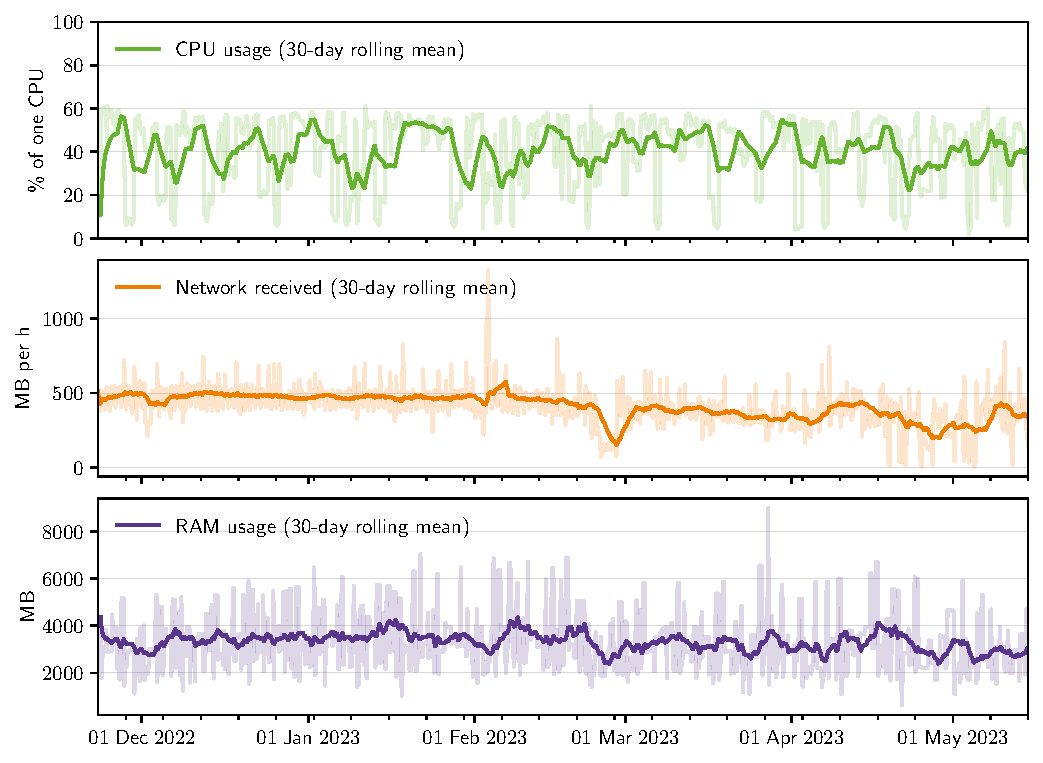
\includegraphics[width=\linewidth]{images/monitoring-prediction-service-load.pdf}
    \caption{Cadvisor statistics for prediction service. Seen here is that the load metrics of the prediction service are within acceptable limits when running the prediction for real-time data of approximately 5000 bike traffic lights.}\label{fig:monitoring-prediction-service-load}
\end{figure}

Based on collected Cadvisor\footnote{\url{https://github.com/google/cadvisor}} metrics on CPU load, RAM usage, and network load, the prediction algorithm scaled well to the multiple thousand traffic lights. The algorithm was implemented in a Java service that also controlled receiving Observations and sending Predictions to our prediction MQTT broker. We measured the service on a TU Dresden server using 6 of 12 cores of an Intel Xeon Gold 6136 CPU running at 3.00 GHz. The CPU percentage utilization of the prediction service was measured via CPU time. As seen in \Cref{fig:monitoring-prediction-service-load}, the service consumes approximately 60\% of the CPU time of a single CPU, translating to around 10\% of the total possible computing capacity when considering the 6 CPUs available on our VM. Both network usage and RAM consumption did also not exceed the capabilities of our VM, meaning that the resource usage was quite low considering the number of messages that were processed every minute.

\begin{figure}[t]
    \centering
    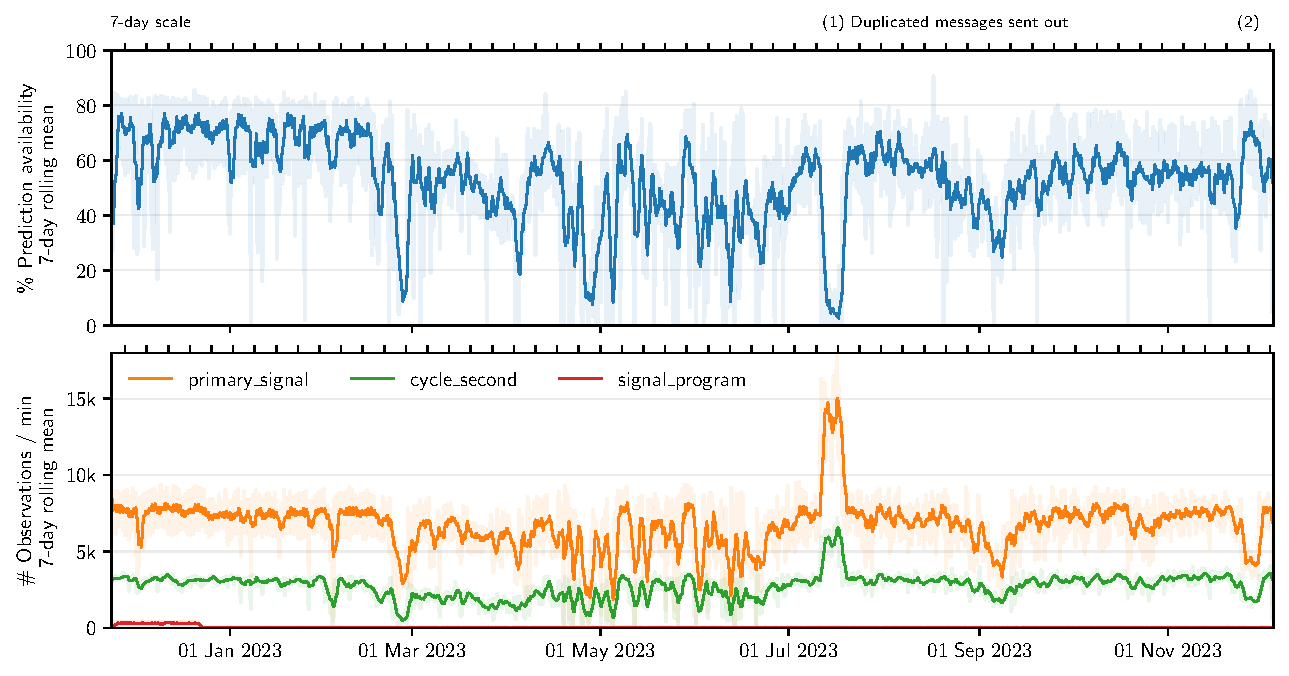
\includegraphics[width=\linewidth]{images/monitoring-availability.pdf}
    \caption{Long-term development of prediction availability. Shown here is for how many traffic lights a prediction was available during 2023, and how drops in availability directly relate to data outages or errors.}\label{fig:monitoring-availability}
\end{figure}

Following this aspect, the long-term data trend and prediction availability are depicted in \Cref{fig:monitoring-availability}. The prediction availability is calculated by dividing the number of predictions generated per minute by the total number of available traffic lights. In the upper part of the figure, we observe that prediction availability typically fluctuates between 40\% and 80\%, with 100\% never being reached. For the period given in the diagram, we calculate a median prediction availability of 55.07\% (IQR: 28.23\%). The maximum observed prediction availability resides at 90.63\%, recorded on September 17, 2023, at 0:00. Thus, the median prediction availability is relatively low throughout the studied period, lower than the minimum of 69\% reported by Protschky et al. (2014) \cite{protschky_extensive_2014, protschky_adaptive_2014} in Munich, while some weeks showed good service availability.

The visible disruptions in prediction availability can be primarily attributed to short-term data errors in the Traffic Lights Data system. For instance, around July 11, 2023 (1), all Observations were accidentally sent twice, causing prediction availability to nearly drop to 0\%. Examining the long-term trend, we notice increased disruptions in prediction availability in the summer of 2023, following an initial period of relatively stable availability. These disruptions coincided with increased maintenance activities on the Traffic Lights Data system, indicating that repeated updates during this period led to a deterioration in data quality. 

Although an increase in prediction availability can be seen around November 23, 2023 (2), this increase originated from us excluding erroneous traffic lights from our prediction service, decreasing the overall number of Observations received. Therefore, the prediction availability over the period under consideration was not optimal.

\begin{figure}[t]
    \centering
    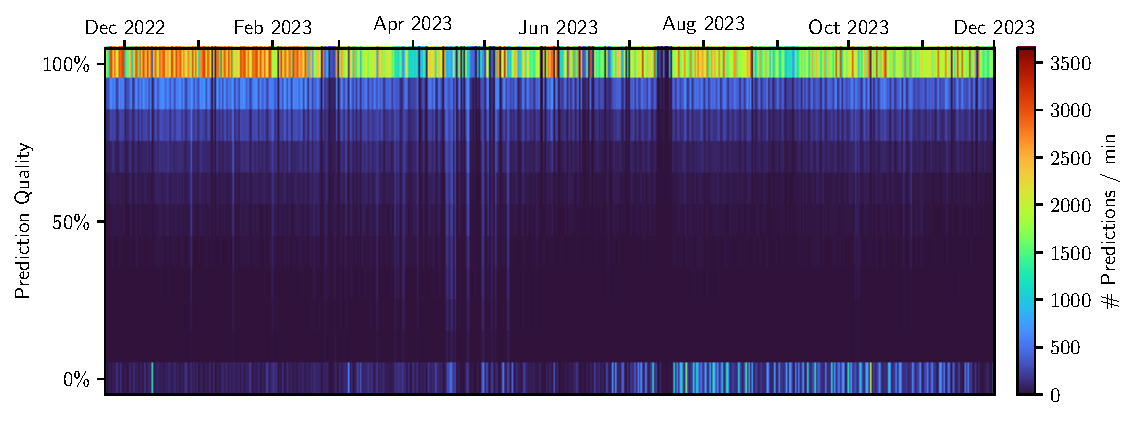
\includegraphics[width=\linewidth]{images/monitoring-long-term-study.pdf}
    \caption{A heatmap displaying the long-term development of prediction quality throughout 2023. The prediction quality was recorded in 10\% buckets for a more responsive analysis in our monitoring tool. In the best case, all predictions should be in the top 10\% bucket. Seen here is how data outages in late 2023 degraded the prediction quality.}\label{fig:monitoring-long-term-study}
\end{figure}

In addition to the prediction availability, we also measured the prediction quality over a longer period. \Cref{fig:monitoring-long-term-study} shows this measurement, mapping prediction qualities of -1 that indicate data outages to the 0\% bucket. 

Considering the 10\% buckets in which the prediction quality was monitored, the calculated median prediction quality resides at 85.78\% (IQR: 1.85\%). At first glance, examining the long-term trend reveals a similar pattern in prediction availability at 100\% quality compared to \Cref{fig:monitoring-availability}. For example, there was also a significant dip around July 11, 2023, due to the duplicated messages issue and a general decrease in availability throughout 2023. In addition, we can see in this diagram that fewer predictions fall within the intermediate 10\% to 90\% quality range. As the increased data outages in the summer of 2023 coincided with an increase in low-quality predictions, most predictions below 10\% are likely due to temporarily missing data. Thus, if interpreted as an accuracy metric, many predictions generated with consistent traffic light data likely have been precise to a few seconds.

\begin{figure}[t]
    \centering
    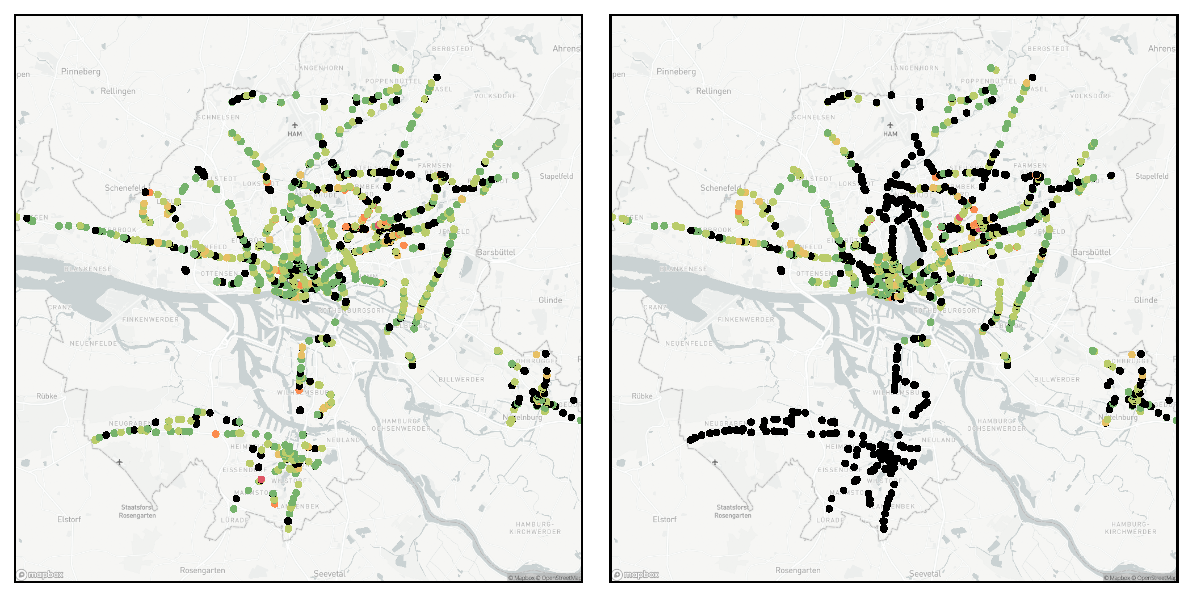
\includegraphics[width=\linewidth]{images/monitoring-before-after-failure.pdf}
    \caption{Before and after traffic controller failure on October 11, 2023. Black predictions indicate outages when the prediction service is unable to verify the prediction quality due to the lack of real-time data. In this case, entire city districts were affected by the outage, pointing to a systematic issue.}\label{fig:monitoring-before-after-failure}
\end{figure}

The decline in prediction availability observed in the summer of 2023 has had multiple origins, many of which could be identified, reported, and addressed through our monitoring tools. The first two kinds of data error that could be pinpointed are highlighted in  \Cref{fig:monitoring-before-after-failure}: blackouts of individual traffic lights (on the left and right) and blackouts affecting entire city districts (on the right only).

Through our map-based prediction quality monitoring, we could help identify 61 intersections and 80 individual connections experiencing persistent issues, rendering them unable to transmit data. In at least 30 cases, a connection was falsely associated with an unsignaled road crossing, or the connection was no longer present. Among 22 nodes, traffic lights utilized the OCIT protocol, which is unsupported by the Traffic Lights Data platform at the time of writing. For 19 nodes, the observed failures are presumed to be construction-related, with this confirmed in three additional cases. In 16 instances, outdated intersection topologies or georeferences were identified. The identified traffic lights were subsequently excluded from the prediction system using an exclude list, with the option to reintegrate them later.

Turning our attention to failures affecting entire city districts, \Cref{fig:monitoring-failure} demonstrates their relatively spontaneous occurrence. This type of failure poses a more significant challenge than individual intersection or connection failures since thousands of predictions are abruptly invalidated. Therefore, we worked rigorously with the platform operators to identify the source of this issue.

\begin{figure}[t]
    \centering
    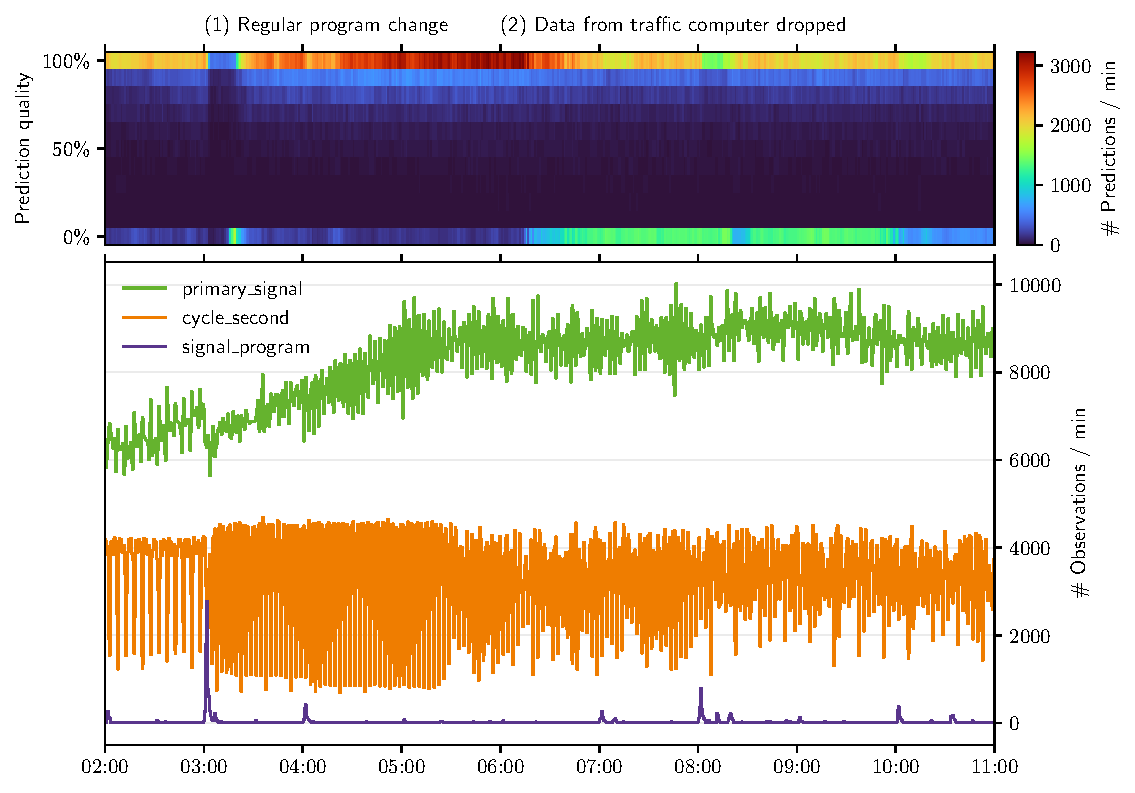
\includegraphics[width=\linewidth]{images/monitoring-failure.pdf}
    \caption{Monitored metrics during traffic controller failure on October 11, 2023. Seen on the bottom are typical patterns of real-time state messages that arrive at the prediction service. Here, no specific issue can be seen. However, the prediction quality heatmap shows a rapid decline in prediction quality that persists for multiple hours. This failure is related to \Cref{fig:monitoring-before-after-failure}.}\label{fig:monitoring-failure}
\end{figure}

To better understand the occurrence of such a failure, we examined the daily data course recorded by our monitoring system, as depicted in \Cref{fig:monitoring-failure}. At 3:00 AM UTC, within the timeline of \texttt{signal\_program} Observations, many traffic lights switch their programs. As confirmed by traffic light operators, this pattern represents the morning program of the weekly automation of the traffic lights being scheduled.

Simultaneously, the availability and quality of the predictions briefly decline (1). This decline can be explained by the fact that the prediction algorithm continues to forecast the old pattern from the previous program for a short period, only synchronizing with the new program after approximately 15 minutes (or ten cycles at 90 seconds). The reason is that the prediction service continues to record cycles and pushes out older cycles from the prediction window only after a few minutes. One identified solution for this issue is to switch between histories recorded for each traffic light once a program Observation arrives.

Following this brief decline, the best prediction quality is achieved around 6:00 AM UTC, just before it suddenly and persistently collapses across multiple districts. The fact that these declines are reflected in specific districts strongly suggests that this issue can be traced back to specific traffic controllers, each generating Observations for one or more districts. 

Once this finding was communicated to the Traffic Lights Data platform operators, it was identified that this problem is indeed associated with specific traffic controllers. The increasing message load throughout the day due to rising traffic causes the message queues of the MQTT brokers at the traffic controllers to fill up. Ultimately, this results in the traffic controllers either not sending messages at all, dropping individual messages, or transmitting them with significant delays.

\begin{figure}[t]
    \centering
    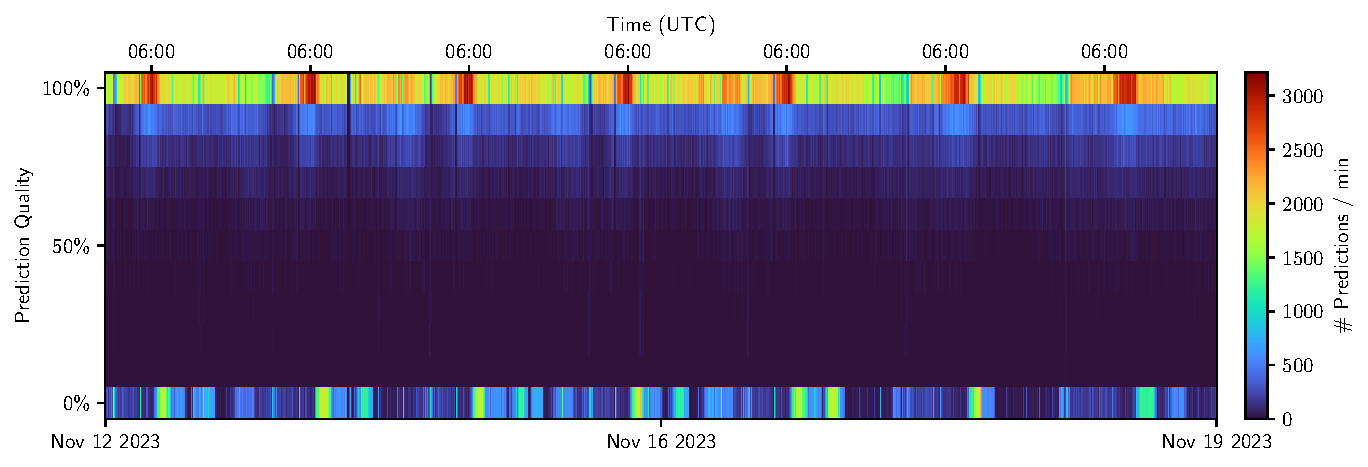
\includegraphics[width=\linewidth]{images/monitoring-7-days.pdf}
    \caption{Heatmap depicting the reoccurring nature of the traffic controller failures after 6:00 UTC. Each time a failure happens, we can see a clear decline in prediction quality, filling up the 0\% bucket.}\label{fig:monitoring-7-days}
\end{figure}

In the weekly progression illustrated in \Cref{fig:monitoring-7-days}, it becomes evident that this situation repeated almost daily at the same hour. Only on Saturdays and Sundays does the issue manifest later, around 7:00 -- 8:00 AM UTC, due to reduced and delayed traffic leading to fewer green phases.

Upon identifying the root cause, the operators initiated appropriate fixes related to the traffic controllers' MQTT queues. Simultaneously, we created an additional exclusion list of intersection nodes, preliminarily exempting them from the prediction until the issue was resolved. This exclusion involved 584 intersections connected to three specific traffic controllers. Due to compliance concerns, the operators have not allowed us to disclose the specific traffic controllers affected; however, further information can be found in a technical report from 2020 \cite{neuner_leitfaden_2020}. 

\begin{figure}[t]
    \centering
    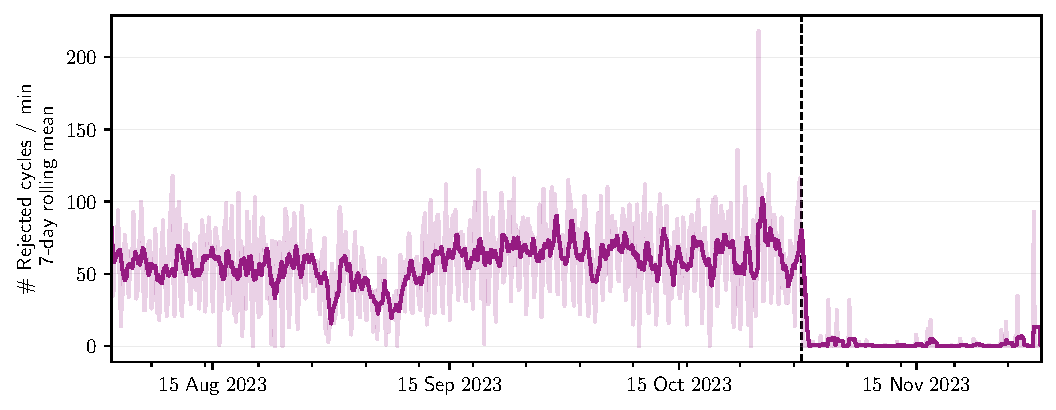
\includegraphics[width=\linewidth]{images/monitoring-rejected-cycles.pdf}
    \caption{Line chart depicting the number of cycles rejected due to out-of-order switching. The clear decline after October 31 at 6:40 AM local time indicates that parts of the traffic light data network infrastructure were fixed, decreasing the number of incomplete cycles.}\label{fig:monitoring-rejected-cycles}
\end{figure}

Looking at the number of discarded cycles, we derive further insights into whether isolated messages are lost or if Observations from operational traffic lights consistently reach their destination. The analysis is depicted in \Cref{fig:monitoring-rejected-cycles} and started around August 1, 2023. After an extended period with invalid cycles, we see a substantial improvement around October 31 at 6:40 AM local time. The number of rejected cycles suddenly dropped to 0, with only sporadic peaks. This improvement indicates that another data issue in the Traffic Lights Data platform was addressed; however, we were not informed which specific modification was made. Before, 25 to 125 cycles were rejected every minute, indicating that the issue could have affected up to 200 connections throughout summer 2023, assuming a cycle length of 90 seconds. At the time of this fix, we had already given Hamburg guest access to our monitoring web tool, meaning it could have been one of the information sources involved in the fix.

After identifying issues with the traffic controllers and falsely importing traffic lights in the data platform, we were also able to identify issues related to the network router installed at the platform operator's servers, which could not keep up with all messages. The corresponding router was replaced, further improving the data quality. The stability of the MQTT brokers directly connected with the traffic controllers was also optimized by scaling up the computational resources of the Observation-exporting virtual machines. As a result of these efforts, the original prediction availability from 2022 (80\% during the day) could be restored in February 2024, stabilizing the Traffic Lights Data system.

\subsection{Study of Traffic Light Predictability in Hamburg}

In the previous section, we found that the prediction availability for traffic lights in Hamburg was low during 2023. However, the core part of this issue could be attributed to data issues. The prediction quality was also likely affected by data issues, as predictions would be invalidated by the missing data, resulting in a prediction quality of -1 (no validation possible) mapped to 0\% in the monitoring. We found that the remaining predictions were mainly centered on 90\% to 100\% quality, more than we expected with the high prevalence of adaptivity-capable traffic lights in Hamburg. This finding was also a key motivation for further investigating the overall predictability of traffic light patterns. 

To conduct these evaluations, we recorded real-time data for four weeks. This recording encompassed 19844 individual traffic lights available in the Traffic Lights Data system at the time of evaluation, including all modes of transport and not only cyclist traffic lights, as in the previous study. During the measurement period, data was obtained from 18009 (90.75\%) of all traffic lights, among which 519 also contained secondary signal data. Thus, although we supplemented the MQTT messages browsing Observations from the Traffic Lights Data platform's HTTP interface, some traffic lights never sent data.

Nonetheless, the supplementation was still effective in addressing partial data outages, as seen in \Cref{fig:adaptiveness-mqtt-http}. On multiple days, approximately half of all recorded Observations were supplemented by the HTTP interface because they were lost preliminarily via MQTT. A minor message dip remained for some days, meaning small parts could not be recovered.


\begin{figure}[t]
    \centering
    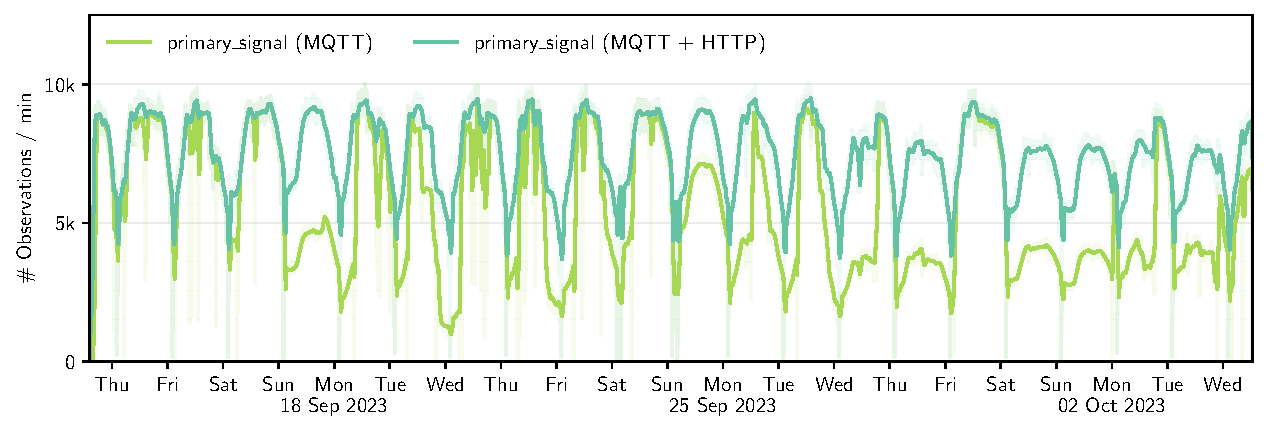
\includegraphics[width=\linewidth]{images/adaptiveness-mqtt-http.pdf}
    \caption{Line chart depicting how many messages were supplemented by browsing through the Traffic Light Data platform's HTTP API, recovering messages that were lost via MQTT.}\label{fig:adaptiveness-mqtt-http}
\end{figure}

The detection of faulty cycles, also implemented in the prediction service, was utilized for problem identification. Out of approximately 424 million reconstructed cycles, 13.8 million cycles were discarded. Here, 90\% of faulty cycles are distributed across 10\% of the connections. One of the known faulty traffic controllers could be identified as the leading cause by examining the faulty connections on the map\footnote{Unfortunately, we cannot disclose the specific traffic controller here due to compliance concerns of authorities in Hamburg, although we would have wished to do so.}. 

These numbers are related to the 40\% of traffic lights that were detected to switch between green, (red-)amber, and red. 34\% of traffic lights that only switched between green and red could also have generated erroneous cycles that were not discarded. The remaining 26\% of traffic lights are comprised of various other switching patterns. The 2106 traffic lights for which an error rate of >10\% was detected were excluded from further analyses.

\begin{figure}[!t]
    \centering
    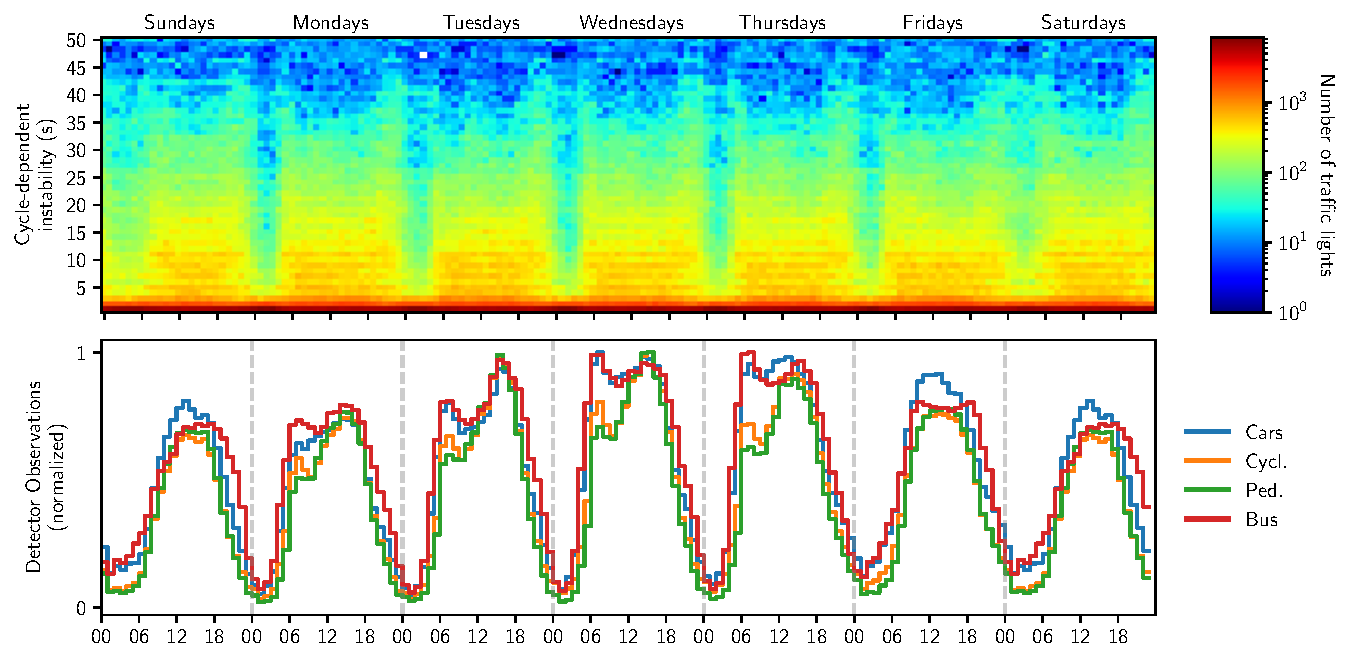
\includegraphics[width=\linewidth]{images/predictability-week-heatmap.pdf}
    \caption{Measured weekly progression of our two predictability metrics, cycle discrepancy and wait time diversity, in relation to the green length and the number of measured green phases throughout the day and the measured traffic volume from vehicle detector Observations. A higher number of vehicle detector Observations indicates a higher traffic density.}\label{fig:adaptiveness-weekdays-distance}
\end{figure}

Thus, we could not eliminate all errors, but they are present only to a minor extent. We assume that the mass of valid data overshadows isolated recording errors. However, it is important to note for subsequent analyses that recording errors may have occurred, e.g., missing cycle Observations leading to multiplied cycle lengths. Accordingly, we will use statistics for evaluation that are robust to outliers.

The first chart displayed in \Cref{fig:adaptiveness-weekdays-distance} looks at the relation between traffic light predictability and daytime. As a statistically robust measure against outliers in the data, we use the median of the cycle discrepancy and wait time diversity for all recorded hourly buckets to analyze how unpredictability evolves during the day. The information and the frequencies of recorded traffic detector Observations are presented to compare the measured predictability to the measured traffic volume.

As a result, predictability decreases, as expected, with increasing traffic volume. While the predictability is at its highest at night, it declines rapidly during the morning traffic surge. This is visible through the increased values in cycle discrepancy and wait time diversity in the heatmap. After the decrease in predictability, it remains relatively constant before increasing again in the evening. It looks like the predictability hits a lower bound, indicating that there may be limits to the adaptiveness even with further increasing traffic. 

When looking closer at the distribution and not only the general trend, the biggest part of traffic lights by one order of magnitude seem not to be influenced by adaptivity at all. As a result, across all traffic lights, the median cycle discrepancy ranges only between 0 and 2 seconds, depending on daytime. The highest median cycle discrepancy during the day comprises only 10\% of the median green length measured at 20 to 23 seconds, meaning that green phases largely overlap between cycles. The wait time diversity shows a similar pattern, although the number of traffic lights with 100\% wait time diversity increases during nighttime. This increase is likely because traffic lights switch to fewer green phases, increasing the chance that the waiting time between green phases is unique.

\begin{figure}[t]
\centering 
\begin{tabular}{@{}cc@{}}
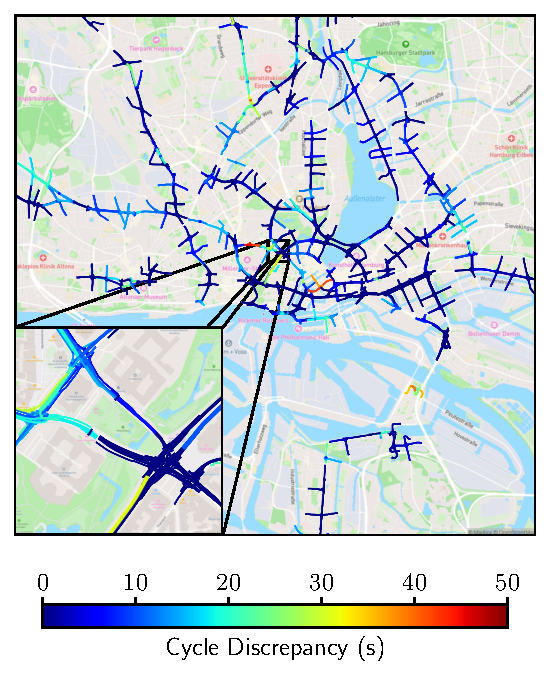
\includegraphics[width=0.46\linewidth]{images/predictability-map.pdf} & 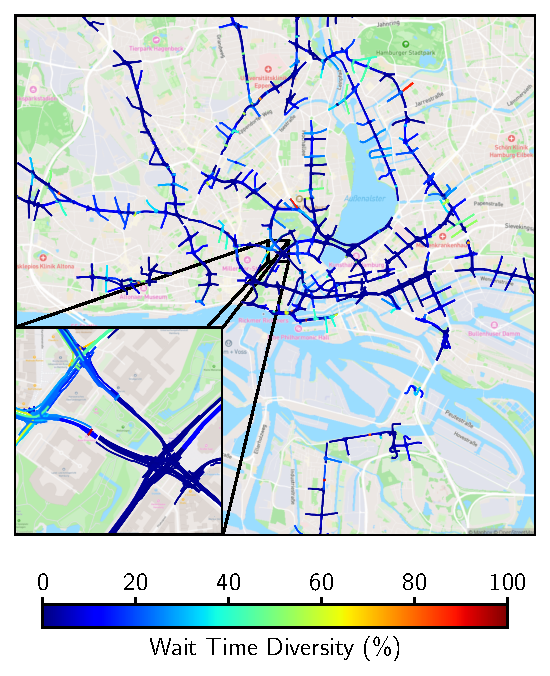
\includegraphics[width=0.46\linewidth]{images/predictability-map-diversity.pdf}
\end{tabular}
\caption{Measured spatial distribution of predictability. Depicted are the traffic light's lanes, colored by their median cycle discrepancy and wait time diversity. Blue parts in the diagram indicate high predictability.} \label{fig:predictability-map}
\end{figure}

\Cref{fig:predictability-map} shows how our predictability metrics are spatially distributed across intersections in Hamburg. While most traffic lights in both images are located in the blue range of the color scale, indicating a high level of predictability, there are a few traffic lights where a higher cycle discrepancy or wait time diversity can be observed. 

As expected, traffic lights with higher unpredictability tend to be located together at the same intersection since they share a joint program and depend on each other's ingress directions. This commonality can be seen in the zoomed-in part of the diagram. However, it can also be seen that traffic lights exhibit only one kind of unpredictability in many cases and not both. Traffic lights exhibiting both unpredictabilities are rare.

\begin{figure}[!t]
    \centering
    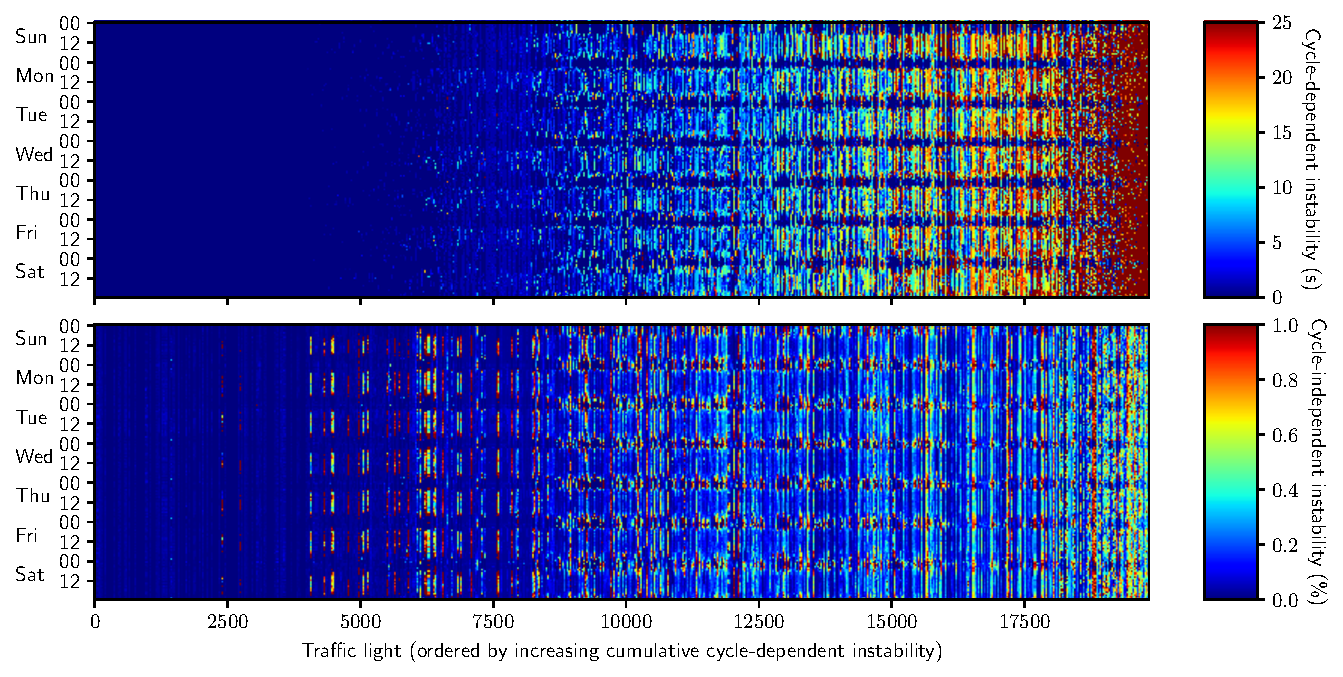
\includegraphics[width=\linewidth]{images/predictability-week-heatmap-per-thing.pdf}
    \caption{Measured weekly progression of both predictability metrics for each traffic light, represented by a vertical line each. Blue parts in the diagram indicate high predictability.}\label{fig:predictability-week-heatmap-per-thing}
\end{figure}

This aspect is explored further in \Cref{fig:predictability-week-heatmap-per-thing}. In the leftmost part of the diagram, traffic lights can be seen that have a low cycle discrepancy but express a high wait time diversity. In the rightmost part, we also find traffic lights with high cycle discrepancy that express low wait time diversity. For these traffic lights, our chosen prediction method may not be ideal. 

Of the evaluated 2,793,786 traffic light hours, 43\% (1,206,817) have a cycle discrepancy of less than 5 seconds and a wait time diversity of less than 10\%. For 67\% of traffic light hours, a cycle discrepancy lower than 5 seconds could be measured, which may also contain higher wait time diversities. Regarding wait time diversity, 77\% of recorded traffic light hours reside below 20\%. Hardly predictable traffic light hours, meaning that the wait time diversity is above 20\% and the cycle discrepancy is above 5 seconds, only comprise 12\% of the overall dataset. Note that the 5-second cycle discrepancy and 20\% wait time diversity were chosen here arbitrarily as a decision boundary, which we felt constituted a good predictability for our scenario. The decision boundary may be chosen more loosely or strictly depending on the prediction accuracy requirements. Nonetheless, the tendency is clear that a large proportion of traffic lights fall into a high predictability (blue) region. 

\begin{figure}[t]
    \centering
    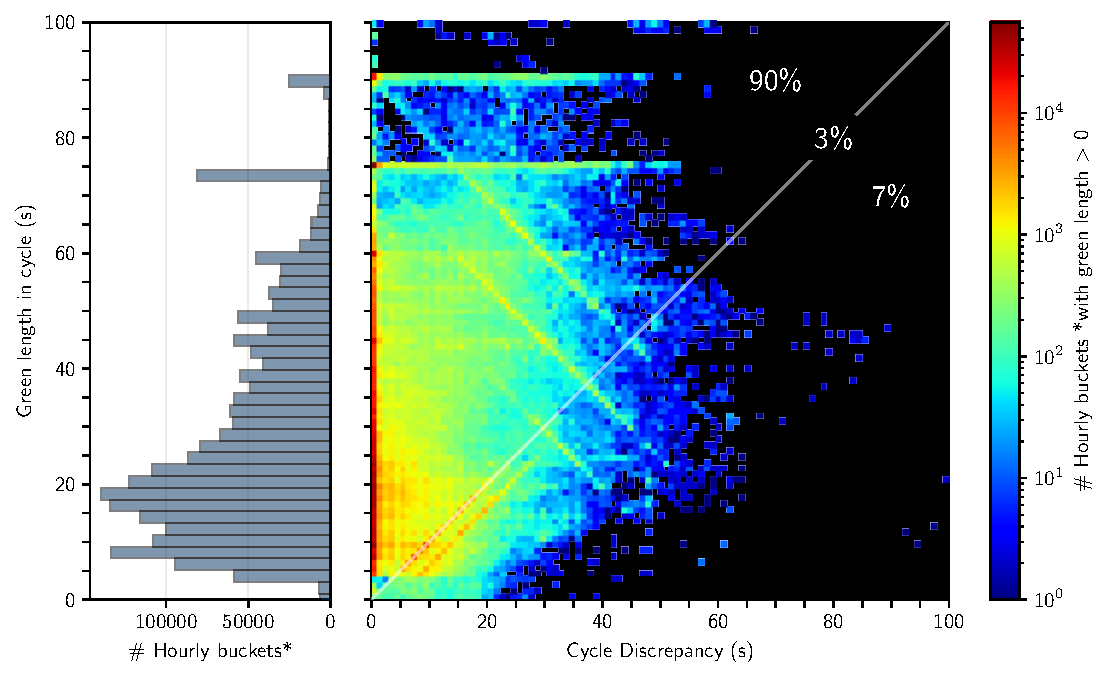
\includegraphics[width=\linewidth]{images/cycle_discrepancy_green_length_heatmap.pdf}
    \caption{Heatmap of the recorded traffic light hours, mapped by their measured green length and cycle discrepancy. Above the depicted diagonal, the cycle discrepancy is shorter than the green length, indicating an overlap of green between cycles and a stable, predictable green phase.}\label{fig:green-length-cycle-discrepancy}
\end{figure}

The results must be viewed in correspondence to the measured green length, which determines how much green overlaps between cycles. Even in the presence of a high cycle discrepancy, a high green overlap would mean that our probabilistic prediction method still finds certain green regions suitable for speed advisory. As seen in \Cref{fig:green-length-cycle-discrepancy} for 90\% of recorded traffic light hours, the median green phase is longer than the median cycle discrepancy. What should be noted here, again, is that most of the traffic light hours reside to the left at a cycle discrepancy of zero seconds. The heatmap colors are scaled logarithmically to reveal more interesting patterns.

Looking more at the revealed patterns may allow us to understand some specific constraints in traffic light behavior. First, a cutoff at 5 seconds of green length can be seen. This follows a best practice of German traffic light planning \cite{TN_libero_mab2}. When extracting and analyzing random examples from specific regions, we find that the horizontal concentrations at 90 seconds, 75 seconds, and 60 seconds primarily stem from traffic lights that switch green for the complete cycle. These buckets are occasionally shifted to the right by red phases of different lengths that interrupt the otherwise switched green phase. Top-left to bottom-right diagonal lines come from traffic lights that extend their green phase until a maximum green duration is reached. Since shorter green phases can be placed more flexibly in the cycle, a decreased green length leads to a higher cycle discrepancy. These constraints could be detected and used to improve the prediction.

\begin{figure}[!t]
    \centering
    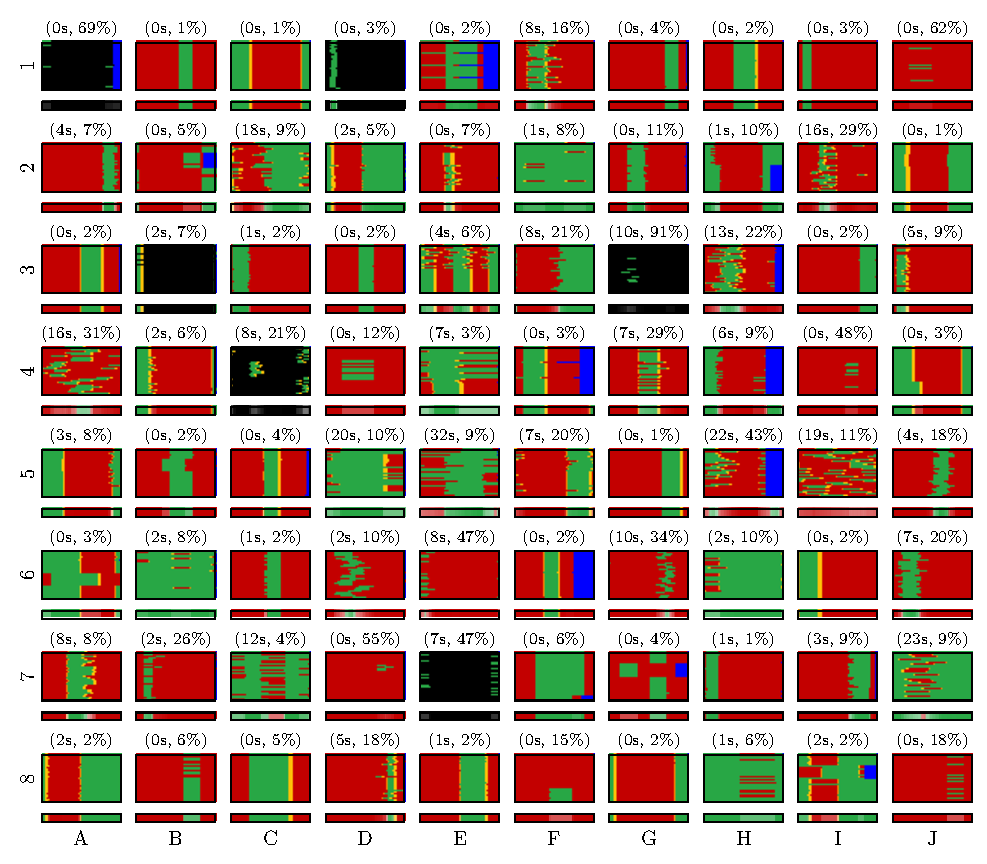
\includegraphics[width=\linewidth]{images/predictability-case-studies.pdf}
    \caption{Random examples of recorded traffic light histories from our database, ordered by their classification according to our two metrics. Below each cycle diagram, a probabilistic prediction based on the cycles is shown. Title format: median (cycle discrepancy, wait time diversity). Low values indicate high predictability. Blue parts of the diagram show cycles that were shorter than the longest recorded cycle during the displayed hour.}\label{fig:types-of-instability}
\end{figure}

To conclude this study, we validate our findings through a random sample of traffic light hours extracted from the recorded database. The extracted sample is highlighted in \Cref{fig:types-of-instability} with the associated values for cycle discrepancy and wait time diversity. Predictions incorporating all cycles in the recorded bucket are also shown to demonstrate how a probabilistic prediction displayed to the user would look. As seen in the visualization, the sample also contains traffic lights that switch between green and black and samples in which the cycle length changed in between, indicated by the blue background.

Overall, most recorded buckets in this sample contain behavior that can be considered predictable. Just looking at the first row, there are already 6 out of 10 cases (B1, C1, E1, G1, H1, I1) with clear columns in the switching pattern that can be easily predicted. There are also cases such as D1, A2, D2, or G2, in which an adaption is visible but limited to a few seconds. In examples such as F2, D5, or H8, we can see traffic lights that are always green until disrupted by a red phase. For cases such as C2, E3, H3, A7, or J7, the traffic adaptivity is more pronounced, as reflected by the high cycle discrepancy score. However, in these cases, as seen before, a joint part in which all cycles are green can still be identified. Examples such as D6 or G6 are more strongly distorted by adaptivity, while these examples also indicate that the green phase centers around a midpoint, as shown in the prediction. An entirely unpredictable pattern is given in I5. As a result, the prediction is fully blurred out. Additionally, with G7, we find one example in which the program seems to have been switched out, indicated by the sudden change in the otherwise stable pattern. Finally, we also see switching behaviors such as E6, J1, J8, or D7, in which the traffic light is switched red most of the time, leading to a red prediction.

While there are examples of apparent adaptive behavior, most recorded switching behaviors contain predictable patterns. This tendency can also be seen in the probabilistic prediction below each cycle diagram, which is only blurred marginally for most predictions. Most predictions contain at least a small fraction of each green phase that is certain. Thus, while highlighting a few interesting examples, our case study generally confirms our previous findings that adaptivity is often only expressed to a minor extent, if at all.

\begin{Summary}[Summary and Discussion of Results]
Our results clearly show that we cannot assume from centralized traffic light data systems that they deliver stable and consistent data. In our case, long-term collaboration with platform operators and active error searching was necessary to stabilize the data system. Previous studies may have been too optimistic here, especially studies that do not work with a real-world system. The highly federated architecture in such systems may lead to complex failure patterns that must be accounted for in the prediction algorithm. 

Through the developed monitoring system, we could identify and help fix multiple systematic issues in Hamburg’s Traffic Lights Data infrastructure, taking over a vital part of the urgently needed quality assurance process. In particular, we could determine a failure pattern related to the traffic controllers that reoccurred daily, helping the operators to scale the data brokers accordingly. Multiple other issues at various parts of the data platform's pipeline were also found and could ultimately be identified and fixed. Even in these harsh circumstances, the probabilistic approach seemed to scale well. It showed good accuracy at most intersections, while the prediction availability was often not optimal due to the described data outages.

Then, we looked at the general predictability of traffic lights in a broader perspective. We found that the predictability decreases during the day, together with the traffic surge, but not as much as expected. We measured that traffic lights switch more adaptively and thus are more unpredictable during the daytime. However, traffic adaptation is minimal for most traffic lights, as predictability only decreases to a limited extent, while many traffic lights remain unaffected. 

Thus, compared to the 90.7\% of traffic lights in Hamburg that should be able to adapt to traffic conditions, we find that this adaptation is only expressed to a minor extent, if at all. Most observed switching patterns align with the cycle length, meaning the probabilistic approach, which highly depends on this alignment, is a good choice. If shifts of the phases in cycles are seen, they are usually shorter than the green time, meaning that some parts of the green phases overlap. This should allow our method to predict green parts of the traffic light switching behavior in most situations with certainty. We confirmed this finding through a randomized case study. Nonetheless, a few intersections were seen at which future experimentation with other methods may be beneficial.
\end{Summary}

\section{Conclusions}

Traffic light prediction provides many opportunities for future intelligent transport systems to enhance the efficiency and safety of traffic, overcoming issues like dilemma zones when approaching an intersection. In practice, however, traffic light prediction is hindered by two issues: obtaining the traffic light data and accounting for unpredictabilities in the switching. 

Previous works mainly resorted to DSRC or cellular V2X to directly obtain traffic light timing information. These systems can use the residual green/red time provided in SPaT messages, externalizing the prediction to the infrastructure provider and ensuring high interoperability between cities. However, as an alternative, we can also use a centralized data platform, making it widely available to all devices with access to the Internet. This solution seems more attractive from a smartphone application's viewpoint. In Hamburg, such a system is available through the Traffic Lights Data platform.

As the Traffic Lights Data platform does not provide traffic light predictions, we needed to interweave an external prediction algorithm based on the available real-time data. To achieve this, we looked for prediction algorithms that are accurate, scalable, and resilient to data outages. A probabilistic approach was identified and integrated based on the available data. To cope with data issues, we implemented a simple error detection that discards erroneous data and degrades the prediction availability in favor of generating fewer false predictions. 

Based on the calculated prediction quality, the developed prediction system works well at most intersections and fulfills our desired capabilities. Only the availability is an issue induced by the frequent data problems. Through a developed monitoring infrastructure, we could help Hamburg's data broker system operators identify reoccurring failures and plan appropriate fixes. From this process, one fundamental conclusion is that employing a centralized traffic light data system may require extensive and continued efforts for data quality assurance. Our monitoring tool was an elemental solution, without which fewer issues would likely have been detected and fixed.

The finding that our prediction algorithm works well stands in contrast to previous works that have repeatedly emphasized the problem of traffic adaptivity. Especially in Hamburg, for which a proportion of 95\% adaptive traffic lights was reported \cite{bodenheimer_enabling_2014} and 90.7\% found based on our research, we expected more significant problems with adverse impacts of traffic adaptivity on our prediction accuracy. Thus, we found a discrepancy between the reported numbers of adaptivity-capable traffic lights and their predictability. 

To investigate this discrepancy further, we spanned a measurement of two unpredictability metrics across Hamburg for four weeks: wait time diversity and cycle discrepancy. The measurements support our finding that only a few traffic lights express adaptivity to a problematic extent for accurate prediction. Most traffic lights express minor shifts, and green phases are often aligned. A few intersections may impose challenges to our chosen prediction algorithm, indicating the need for experimentation with other prediction methods.

Although the established prediction system can be considered a sound foundation for our bike-GLOSA system that circumvented many issues and contributed to the overall understanding of real-world traffic light predictability, there are also open questions for future work. One issue is a lack of ground truth for traffic light messages. Momentarily, we must trust that the traffic light messages contain the correct timing and state information. However, traffic lights sending false timestamps can be a real problem, potentially resulting in a confident prediction that does not reflect the real-world situation. To address this issue, we could think of inferring traffic lights sending invalid data, for example, from user trajectories. 

Even with minor adaptivity, there could still be situations in which the speed advisory is false, requiring users always to pay attention themselves. Calculating probabilities for each second in the prediction is one step in the right direction, ensuring higher trustworthiness and less fluctuation in the speed advisory. However, there are many more steps to go until a prediction can be considered 100\% trustworthy. A more direct collaboration between the prediction system and the internal program switching in traffic lights is needed to attain such a goal, and a history-based prediction may not suffice. In the presence of recent developments in more connected and adaptive traffic control systems, the prediction of traffic lights may become much more challenging in the future.

What remains open is some experimentation with other prediction models on the intersections that have shown low predictability. In our context, we assumed that users could accept a few missing intersections, considering that the prediction turns itself off with highly adaptive traffic lights. That Machine Learning models could be significantly more accurate than a simple probabilistic approach is clear. However, the question is whether these models could also generate a more accurate prediction, considering that poor predictability often arises from erroneous or unavailable data. The resilience of these models against these data issues should be studied further. Latencies in the data and the needed computational resources to predict multiple thousand traffic lights are also key. Future work should focus on this relation to determine under which conditions which model is the most practical.
